\documentclass[a4paper]{article}
\usepackage{pgf,tikz,pgfplots}
\usetikzlibrary{arrows,decorations.markings}
\pgfplotsset{compat=1.15}
\usepackage{mathrsfs}
\usetikzlibrary{arrows}
%% Language and font encodings
\usepackage[english]{babel}
\usepackage[utf8x]{inputenc}
\usepackage[T1]{fontenc}
\usepackage{float}
%% Sets page size and margins
\usepackage[a4paper,top=3cm,bottom=2cm,left=3cm,right=3cm,marginparwidth=1.75cm]{geometry}
\usepackage{fancyhdr}
\pagestyle{fancy}
%% Useful packages
\usepackage{tensor}
\usepackage{xcolor}
\usepackage{color,soul}
\usepackage{amsmath}
\usepackage{amsthm}
\usepackage{enumitem}
\usepackage{eqnarray}
\usepackage{float}
\usepackage{esint}
\usepackage{wrapfig}
\usepackage{gensymb}
\usepackage{lipsum}
\usepackage{amssymb}
\usepackage{array}
\usepackage{tikz}
\usepackage[colorlinks=true, allcolors=blue]{hyperref}
\usepackage{graphicx}
\usepackage{amsmath}
\usepackage{amssymb}
\usepackage{graphicx}
\usepackage[colorlinks=true, allcolors=blue]{hyperref}
\usepackage{mathtools}
\DeclareMathOperator{\Proj}{Proj}
\DeclareMathOperator{\lcm}{lcm}
\DeclareMathOperator{\cosec}{cosec}
\DeclareMathOperator{\sgn}{sgn}
\DeclareMathOperator{\Span}{span}
\DeclareMathOperator{\nullity}{nullity}
\DeclarePairedDelimiter\floor{\lfloor}{\rfloor}
\DeclareMathOperator{\Res}{Res}
\DeclareMathOperator{\rank}{rank}
\DeclareMathOperator{\Ker}{Ker}
\DeclareMathOperator{\R}{R}
\DeclareMathOperator{\Tr}{Tr}
\DeclareMathOperator{\diag}{diag}
\DeclareMathOperator{\Log}{Log}
\DeclareMathOperator{\sech}{sech}
\DeclareMathOperator{\Var}{Var}
\newtheoremstyle{new2}% <name>
{2pt}% <Space above>
{2pt}% <Space below>
{\color{black}}% Body font
{}% <Indent amount>
{\bfseries\color{black}}% Theorem head font
{:}% <Punctuation after theorem head>
{.5em}% <Space after theorem headi>
{}% <Theorem head spec (can be left empty, meaning `normal')>
\theoremstyle{new2}
\newtheorem{ans}{Answer}[section]
\usetikzlibrary{decorations.markings}
\tikzset{->-/.style={decoration={
  markings,
  mark=at position #1 with {\arrow{>}}},postaction={decorate}}}
\tikzset{-<-/.style={decoration={
  markings,
  mark=at position #1 with {\arrow{<}}},postaction={decorate}}}
\newcommand{\highlight}[1]{%
  \colorbox{red!50}{$\displaystyle#1$}}
  
\definecolor{darkblue}{RGB}{	0, 0, 139}
\newtheoremstyle{new}% <name>
{2pt}% <Space above>
{2pt}% <Space below>
{\color{darkblue}}% Body font
{}% <Indent amount>
{\bfseries\color{black}}% Theorem head font
{:}% <Punctuation after theorem head>
{.5em}% <Space after theorem headi>
{}% <Theorem head spec (can be left empty, meaning `normal')>
\theoremstyle{new}
\newtheorem{qns}{Problem}[section]
\setlength{\parindent}{0cm}
\title{\textbf{Part II AFD Problem Sheet Solutions}}
\author{Tai Yingzhe, Tommy (ytt26)}
\date{}
\setlength{\parindent}{0cm}
\begin{document}
\maketitle
\tableofcontents
\subsection*{Acknowledgements:}
Many thanks to my supervisor Sergei Dyda for their guidance.
\newpage
\section{Problem Sheet 1}
\begin{qns}[Streamline]
Determine the equation of a general streamline of the flow $u_\phi = a$, $u_R = b$, $u_Z = 0$ in cylindrical polar coordinates, and sketch the flow. Include more than one streamline in your sketches. Repeat for the flow $u_\phi = aR^2$, $u_R = bR^2$, $u_Z = 0$. If the flows are steady, and the density at a given radius is independent of $\phi$, find the radial dependence of the density in both cases.
\end{qns}
\begin{ans}
The streamline condition is
$$\frac{d\mathbf{r}}{ds}\times\mathbf{u}=\boldsymbol{0}\implies\frac{dR}{u_R}=\frac{Rd\phi}{u_\phi}\implies R\propto\exp(b\phi/a)$$
where the proportionality constant depends on the boundary conditions. The streamlines spiral outwards since the radius increases exponentially with the plane polar phase, here assume $b/a>0$. 
\begin{center}
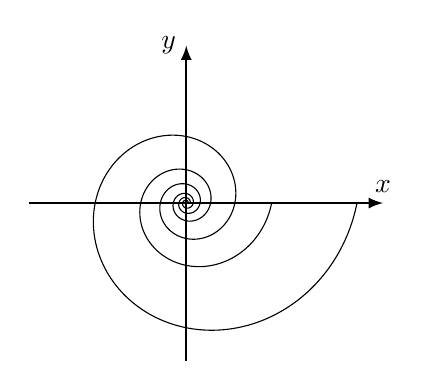
\begin{tikzpicture}
  \draw[thick,->,>=latex] (-2,0)--(2.5,0) node[above] {$x$};
  \draw[thick,->,>=latex] (0,-2)--(0,2) node[left] {$y$};
  \draw[domain=0:6*pi,scale=0.25,samples=500] plot ({deg(\x)}:{0.1*exp(0.2*\x)});
  \draw[domain=0:6*pi,scale=0.25,samples=500] plot ({deg(\x)}:{0.2*exp(0.2*\x)});
\end{tikzpicture}
\end{center}
Similarly, we have
$$\frac{dR}{bR^2}=\frac{Rd\phi}{aR^2}\implies\frac{dR}{R}=\frac{b}{a}d\phi\implies R\propto\exp(b\phi/a)$$
hence, the same streamlines as before. The continuity equation for steady flow is $\boldsymbol{\nabla}\cdot(\rho\mathbf{u})=0$. For cylindrical polar coordinates, we have
$$0=\rho\bigg(\frac{1}{R}\frac{\partial Ru_R}{\partial R}+\frac{1}{R}\frac{\partial u_\phi}{\partial\phi}\bigg)+u_R\frac{d\rho}{dR}$$
We are given $\rho=\rho(R)$, so for the two cases, we have
\begin{itemize}
    \item 
    $$-\mathbf{u}\cdot\boldsymbol{\nabla}\rho=\rho\boldsymbol{\nabla}\cdot\mathbf{u}=\rho\bigg(\frac{1}{R}\frac{\partial Rb}{\partial R}+\frac{1}{R}\frac{\partial a}{\partial\phi}\bigg)=\frac{\rho b}{R}\implies\frac{d\rho}{dR}=-\frac{\rho}{R}\implies\rho\propto\frac{1}{R}$$
    \item 
    $$-\mathbf{u}\cdot\boldsymbol{\nabla}\rho=\rho\boldsymbol{\nabla}\cdot\mathbf{u}=\rho\bigg(\frac{1}{R}\frac{\partial R^3b}{\partial r}+\frac{1}{R}\frac{\partial aR^2}{\partial\phi}\bigg)=3Rb\rho\implies\frac{d\rho}{dR}=-\frac{3\rho}{R}\implies\rho\propto\frac{1}{R^3}$$
\end{itemize}

\end{ans}
\begin{qns}[Streamline]
Show that for a steady flow with $\boldsymbol{\nabla}\cdot\mathbf{u}=0$, the density $\rho$ is constant along the streamlines. Need $\rho$ be constant throughout the medium?
\end{qns}
\begin{ans}
The continuity equation for steady incompressible flow is
$$\boldsymbol{\nabla}\rho\cdot\mathbf{u}=0$$
i.e. $\boldsymbol{\nabla}\rho$ component along direction of $\mathbf{u}$ must be zero, hence $\rho$ is constant along the streamlines. But of course, the component of $\boldsymbol{\nabla}\rho$ perpendicular to $\mathbf{u}$ will give zero even if $\boldsymbol{\nabla}\rho\neq \boldsymbol{0}$. Hence, $\rho$ does not need to be constant throughout the medium.
\end{ans}
\newpage
\begin{qns}[Streamline]
If $\mathbf{R} = (x, y, 0)$ and $\mathbf{\hat{R}} =\frac{\mathbf{R}}{|\mathbf{R}|}$ and a flow velocity is given for $R\geq a$ by $u = U\mathbf{\hat{x}}(1+ \frac{a^2}{R^2})−2U a^2xR^{-3}\mathbf{\hat{R}}$ (where $\mathbf{\hat{x}}=\frac{\mathbf{x}}{|\mathbf{x}|}$) show that the streamlines obey $U(R-\frac{a^2}{R})\sin\phi$= constant [where $\phi=\tan^{-1}\frac{y}{x}$]. Sketch the streamlines and explain what the flow represents physically. [Hint: consider which coordinate system is better suited for this problem.]
\end{qns}
\begin{ans}
We convert the Cartesian coordinate system to polar coordinate system
$$\mathbf{\hat{R}}=\cos\phi\mathbf{\hat{x}}+\sin\phi\mathbf{\hat{y}},\quad\boldsymbol{\hat{\phi}}=-\sin\phi\mathbf{\hat{x}}+\cos\phi\mathbf{\hat{y}}\implies\mathbf{\hat{x}}=\cos\phi\mathbf{\hat{R}}-\sin\phi\boldsymbol{\hat{\phi}}$$
The velocity is then
$$\mathbf{u}=U\bigg(1-\frac{a^2}{R^2}\bigg)\cos\phi\mathbf{\hat{R}}-U\bigg(1+\frac{a^2}{R^2}\bigg)\sin\phi\boldsymbol{\hat{\phi}}=U\bigg(1+\frac{a^2}{R^2}\bigg)\mathbf{\hat{x}}-2Ua^2\frac{R\cos\phi}{R^3}(\cos\phi\mathbf{\hat{x}}+\sin\phi\mathbf{\hat{y}})$$
The streamlines are
$$\frac{d\mathbf{r}}{ds}\times\mathbf{u}=\boldsymbol{0}\implies\frac{dR}{u_R}=\frac{Rd\phi}{u_\phi}\implies\frac{dR}{U(1-(a^2/R^2))\cos\phi}=\frac{Rd\phi}{-U(1+(a^2/R^2))\sin\phi}$$
which gives the exact differential:
$$0=U\bigg(1+\frac{a^2}{R^2}\bigg)\sin\phi dR+U\bigg(R-\frac{a^2}{R}\bigg)\cos\phi d\phi=d\bigg(U\bigg(R-\frac{a^2}{R}\bigg)\sin\phi\bigg)$$
The streamlines thus obey $U(R-\frac{a^2}{R})\sin\phi=$const. The flow velocity can be rewritten as
$$\mathbf{u}=U\bigg(1+\frac{a^2}{R^2}\bigg)-2U\frac{a^2}{R^2}\cos^2\phi\mathbf{\hat{x}}-\frac{Ua^2}{R^2}\sin2\phi\mathbf{\hat{y}}=U\mathbf{\hat{x}}-U\frac{a^2}{R^2}\bigg(\cos2\phi\mathbf{\hat{x}}+\sin2\phi\mathbf{\hat{y}}\bigg)$$
which is a superposition of a constant flow and a flow that falls off as $1/r^2$.
\begin{center}
  \begin{center}
    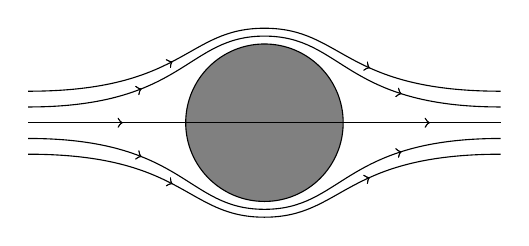
\begin{tikzpicture}
      \draw [fill=gray] circle [radius=1];
      \draw [->-=0.2, ->-=0.85] (-3, 0) -- (3, 0);
      

      \draw [->-=0.23, ->-=0.8] (-3, 0.2) .. controls (-1, 0.2) and (-1, 1.1) .. (0, 1.1) .. controls (1, 1.1) and (1, 0.2) .. (3, 0.2);
      \draw [->-=0.3, ->-=0.73] (-3, 0.4) .. controls (-1, 0.4) and (-1, 1.2) .. (0, 1.2) .. controls (1, 1.2) and (1, 0.4) .. (3, 0.4);
      \draw [->-=0.23, ->-=0.8] (-3, -0.2) .. controls (-1, -0.2) and (-1, -1.1) .. (0, -1.1) .. controls (1, -1.1) and (1, -0.2) .. (3, -0.2);
      \draw [->-=0.3, ->-=0.73] (-3, -0.4) .. controls (-1, -0.4) and (-1, -1.2) .. (0, -1.2) .. controls (1, -1.2) and (1, -0.4) .. (3, -0.4);
    \end{tikzpicture}
  \end{center}
\end{center}
\end{ans}
\newpage
\begin{qns}[Streamline]
A steady 2D flow is described by $u_x=\frac{2}{x}$, $u_y = 1$. Find and sketch the streamlines. Find also a general expression for the surface density of the flow $\Sigma(x, y)$ assuming it can be written as a separable function of $x$ and $y$. Radioactive nuclei are introduced in a small patch at $(x_0, y_0)$ so as to maintain a fixed concentration there. These nuclei decay such that their number per unit mass is given by $Q=Q_0e^{-t}$ where $t$ is the time since introduction into the flow. Show that the surface density of radioactive nuclei (i.e. number per unit area) attains a maximum along the radioactive streakline if $x_0$ is less than a critical value, and determine the coordinates of this maximum.
\end{qns}
\begin{ans}
The streamlines are
$$\frac{d\mathbf{r}}{ds}\times\mathbf{u}=\boldsymbol{0}\implies\frac{dx}{u_x}=\frac{dy}{u_y}\implies \frac{dx}{2/x}=dy\implies y=\frac{x^2}{4}+c$$
i.e. parabolic streamlines. Since the flow is steady, the streamlines are the same as the streaklines, which may be parametrized by the equation $y-y_0=0.25(x^2-x_0^2)$, where $(x_0,y_0)$ at $t=0$.
\begin{center}
\begin{tikzpicture}
      \draw[->] (-3,0) -- (3,0) node[right] {$x$};
      \draw[->] (0,-1) -- (0,3.5) node[left] {$y$};
      \draw[domain=-1.5:1.5,smooth,variable=\x,black] plot ({\x},{\x*\x)});
      \draw[domain=-1.5:1.5,smooth,variable=\x,black] plot ({\x},{\x*\x+1)});
      \draw[domain=-1.5:1.5,smooth,variable=\x,black] plot ({\x},{\x*\x-1)});
      \draw (0,0) node[below]{0};
\end{tikzpicture}
\end{center}
The continuity equation for a steady flow is
$$\boldsymbol{\nabla}\cdot(\Sigma\mathbf{u})=0$$
where $\Sigma(x,y)$ is the surface density of the flow. Assume $\Sigma(x,y)=X(x)Y(y)$ has a separable form:
$$0=\frac{\partial\Sigma}{\partial x}u_x+\frac{\partial\Sigma}{\partial y}u_y+\Sigma\frac{\partial u_x}{\partial x}+\Sigma\frac{\partial u_y}{\partial y}=X'\frac{2}{x}Y+Y'X-XY\frac{2}{x^2}\implies\frac{2}{X}\frac{d}{dx}\frac{X}{x}=-\frac{1}{Y}\frac{dY}{dy}=\lambda$$
where $\lambda$ is a constant, giving $Y(y)\propto e^{-\lambda y}$ and $X(x)\propto xe^{\lambda x^2/4}$ $\implies \Sigma(x,y)=Cxe^{-\lambda y}e^{\lambda x^2/4}$. The number per unit mass is $Q=Q_0e^{-t}$ and so the surface density, which is mass per unit area, gives the number per unit area to be $Q\Sigma$. We have
$$u_y=1\implies y=y_0+t\implies t=y-y_0=\frac{1}{4}(x^2-x_0^2)$$
$$\implies Q\Sigma\propto xe^{-\lambda(y_0+0.25(x^2-x_0^2))}e^{\lambda x^2/4}e^{-(x^2-x_0^2)/4}\propto xe^{-x^2/4}$$
The maximum number per unit area along a streakline occurs when $\frac{d}{dx}Q\Sigma=0$ at $x=x_{\text{max}}$, i.e.
$$0=x_{\text{max}}(-x_{\text{max}}/2)e^{-x^2/4}+e^{-x^2/4}\implies x_{\text{max}}=\pm\sqrt{2},~y_{\text{max}}=y_0+\frac{1}{2}-\frac{x_0^2}{4}$$
Following the direction of streaklines, we require $|x_0|<\sqrt{2}=x_{\text{max}}$, in order for the streakline to pass through the point of maximum surface density.
\end{ans}
\newpage
\begin{qns}[Fluid equations]
Use the summation convention to prove:
\begin{enumerate}[label=(\alph*)]
\item $\mathbf{b}\times\boldsymbol{\nabla}\times\mathbf{b}=\boldsymbol{\nabla}(\frac{1}{2}\mathbf{b}\cdot\mathbf{b})-\mathbf{b}\cdot\boldsymbol{\nabla}\mathbf{b}$
\item $\boldsymbol{\nabla}\times(\boldsymbol{\nabla}a)=0$
\item $\boldsymbol{\nabla}\times(a\mathbf{b})=a\boldsymbol{\nabla}\times\mathbf{b}-\mathbf{b}\times\boldsymbol{\nabla}a$. 
\end{enumerate}
Using the above identities and the curl of the momentum equation, show that if $\boldsymbol{\nabla}\times\mathbf{u}=\boldsymbol{0}$ everywhere at time $t = t_0$, then it remains so provided that the pressure is a function of the density only.
\end{qns}
\begin{ans}\leavevmode
\begin{enumerate}[label=(\alph*)]
\item 
$$\varepsilon_{ijk}b_i\varepsilon_{pqj}\partial_pb_q=(\delta_{kp}\delta_{iq}-\delta_{kq}\delta_{ip})b_i\partial_pb_q=b_i\partial_kb_i-b_i\partial_ib_k=\frac{1}{2}\partial_k(b_ib_i)-b_i\partial_ib_k$$
\item $\varepsilon_{ijk}\partial_i\partial_ja$ is a contraction of a tensor anti-symmetric in indices $i,j$ and another tensor symmetric in $i,j$, and hence evaluate to zero.
\item 
$$\varepsilon_{ijk}\frac{\partial}{\partial x_i}(ab_j)=\varepsilon_{ijk}\bigg[a\frac{\partial b_j}{\partial x_i}-b_i\frac{\partial a}{\partial x_j}\bigg]$$
where in the second term $i,j$ are dummy indices.
\end{enumerate}
We start from the momentum equation. From (a),
$$-\frac{1}{\rho}\boldsymbol{\nabla}p+\mathbf{g}=\frac{\partial\mathbf{u}}{\partial t}+(\mathbf{u}\cdot\boldsymbol{\nabla})\mathbf{u}=\frac{\partial\mathbf{u}}{\partial t}+\boldsymbol{\nabla}\frac{1}{2}|\mathbf{u}|^2-(\mathbf{u}\times\boldsymbol{\nabla}\times\mathbf{u})$$
Now take the curl, noting that $\mathbf{g}=-\boldsymbol{\nabla}\Phi$ ($\Phi$ is the gravitational potential):
$$\frac{\partial}{\partial t}(\boldsymbol{\nabla}\times\mathbf{u})+\boldsymbol{\nabla}\times\boldsymbol{\nabla}\frac{1}{2}|\mathbf{u}|^2-\boldsymbol{\nabla}\times\mathbf{u}\times\boldsymbol{\nabla}\times\mathbf{u}=-\frac{1}{\rho}\boldsymbol{\nabla}\times\boldsymbol{\nabla}p-\boldsymbol{\nabla}p\times\boldsymbol{\nabla}\rho^{-1}-\boldsymbol{\nabla}\times\boldsymbol{\nabla}\Phi$$
where we used the result of (c), when we take the curl of $\rho^{-1}\boldsymbol{\nabla}p$. But from (b), the curl of a gradient is zero and we have
$$\frac{\partial}{\partial t}(\boldsymbol{\nabla}\times\mathbf{u})-\boldsymbol{\nabla}\times\mathbf{u}\times\boldsymbol{\nabla}\times\mathbf{u}=\boldsymbol{\nabla}p\times\frac{1}{\rho^2}\boldsymbol{\nabla}\rho$$
Suppose $p=p(\rho)$ (given), then $\boldsymbol{\nabla}p=\frac{dp}{d\rho}\boldsymbol{\nabla}\rho$, hence $\boldsymbol{\nabla}p\times\boldsymbol{\nabla}\rho=\frac{dp}{d\rho}\boldsymbol{\nabla}\rho\times \boldsymbol{\nabla}\rho=\boldsymbol{0}$. Hence,
$$\frac{\partial}{\partial t}(\boldsymbol{\nabla}\times\mathbf{u})=\boldsymbol{\nabla}\times(\mathbf{u}\times(\boldsymbol{\nabla}\times\mathbf{u}))$$
so if $\boldsymbol{\nabla}\times\mathbf{u}=\boldsymbol{0}$ at $t=t_0$, we must have $\boldsymbol{\nabla}\times\mathbf{u}$ to be a constant at all times, specifically remaining zero.
\end{ans}
\newpage
\begin{qns}[Gravitation]
A static infinite slab of incompressible self-gravitating fluid of density $\rho$ occupies the region $|z| < a$. Find the gravitational field everywhere and the pressure distribution within the slab. [Hint: check the limits when integrating the pressure gradient.]\\[5pt]
If a galactic disk is approximated by a uniform density slab with density $10^{−18}$ kg m$^{−3}$ and $a =10^{18}$ m, determine the velocity of a star at the midplane if it starts from rest at $z = a$, and the period of its oscillation.
\end{qns}
\begin{ans}
To find the gravitational field everywhere, we use Gauss' law for gravitation. Inside the slab ($|z|<a$):
$$\int\mathbf{g}\cdot d\mathbf{S}=-4\pi GM\implies -2A|\mathbf{g}|=-4\pi G\int_{-z}^z\rho Adz\implies|\mathbf{g}|=4\pi G\rho z$$
but outside the slab ($|z|>a$):
$$|\mathbf{g}|=4\pi G\rho a$$
Gravity is attractive, so $\mathbf{g}$ points towards $z=0$. To find the pressure within the slab, we use the momentum equation for a static fluid:
$$0=\frac{D\mathbf{u}}{Dt}=-\rho\boldsymbol{\nabla}p+\mathbf{g}\implies\frac{dp}{dz}=-4\pi G\rho^2z$$
where we consider inside the slab. Integrating it gives
$$\int_{p_0}^0dp=-\int_0^a4\pi G\rho^2zdz\implies p_0=2\pi\rho^2Ga^2\implies\int_{p_0}^pdp=-\int_0^z4\pi G\rho^2zdz$$
where the boundary condition is $p=0$ on the surface $z=a$ and the pressure at the centre is $p_0$. This gives $p=2\pi\rho^2G(a^2-z^2)$. The star experiences gravitational acceleration
$$-4\pi G\rho z=g=\frac{du}{dt}=u\frac{du}{dz}\implies\int_0^{u_0}udu=-4\pi G\rho\int_a^0zdz\implies u_0=\pm\sqrt{4\pi G\rho a^2}$$
which gives $u_0=3\times10^4$ m/s towards $z=0$, for $\rho=10^{-18}$ kg m$^{-3}$ and $a=10^{18}$ m. The star undergoes simple harmonic motion about the midplane:
$$\ddot{z}=-4\pi G\rho z\implies T=\frac{2\pi}{\sqrt{4\pi G\rho}}$$
which is the period of oscillation and it gives $T=2.17\times10^{14}$ s, which is about 7 million years.
\end{ans}
\newpage
\begin{qns}[Gravitation]
A stellar wind behaves as a steady adiabatic spherical outflow of a perfect monatomic gas (so $\gamma=c_p/c_v=5/3$) from the surface of the star, so at radius a the density is $\rho_0$, temperature $T_0$, and outflow velocity $u_0$. If the fluid motions are dominated by the star’s gravitational potential, determine the temperature as a function of the radius from the star centre.\\[5pt] 
If the flow velocity $u_0$ at radius $a$ is just the gravitational escape velocity from that point do pressure effects ever become significant?
\end{qns}
\begin{ans}
Momentum equation for a steady flow is
$$\rho\mathbf{g}=\rho(\mathbf{u}\cdot\boldsymbol{\nabla})\mathbf{u}=\rho u\frac{du}{dr}$$
Invoke Gauss' law of gravity and spherical symmetry:
$$4\pi GM=-4\pi r^2g$$
for $r>a$, where $M$ is the mass of the star. We then have
$$u\frac{du}{dr}=-\frac{GM}{r^2}\implies\frac{1}{2}(u^2-u_0^2)=-GM\bigg(\frac{1}{a}-\frac{1}{r}\bigg)\implies u=\sqrt{2GM(1/r-1/a)+u_0^2}$$
The continuity equation for a steady flow is
$$0=\boldsymbol{\nabla}\cdot(\rho\mathbf{u})=\frac{1}{r^2}\frac{\partial}{\partial r}(r^2\rho u)$$
where we invoked spherical symmetry, hence $r^2\rho u=a^2\rho_0u_0$, which is a constant. To find temperature, we use the adiabatic condition $p\propto T^{\gamma/(\gamma-1)}\propto\rho^\gamma$ for $\gamma=5/3$, which gives 
$$T=\frac{T_0}{\rho_0^{\gamma-1}}\rho^{\gamma-1}=\frac{T_0}{\rho_0^{\gamma-1}}\bigg(\rho_0\frac{a^2u_0}{r^2u}\bigg)^{\gamma-1}=T_0\bigg(\frac{a^2u_0}{r^2}\bigg)^{\gamma-1}u^{1-\gamma}=T_0\bigg(\frac{a^2u_0}{r^2}\bigg)^{2/3}u^{-2/3}$$
$$\implies T=T_0\bigg(\frac{a^2u_0}{r^2}\bigg)^{2/3}\bigg[2GM\bigg(\frac{1}{a}-\frac{1}{r}\bigg)+u_0^2\bigg]^{-1/3}$$
The escape velocity is $u_0=\sqrt{2GM/a}$. Inspect the momentum equation, we have
$$\rho=\frac{a^2u_0\rho_0}{r^2u}=\frac{a^2u_0\rho_0}{r^2}\bigg[2GM\bigg(-\frac{1}{a}+\frac{1}{r}\bigg)+\frac{2GM}{a}\bigg]^{-1/2}=\bigg(\frac{a}{r}\bigg)^2\sqrt{2GM/a}\sqrt{r/2GM}\rho_0\propto\frac{1}{r^{3/2}}$$
Assume equation of state of the form $p\propto\rho^\gamma$, then
$$\frac{1}{\rho}\frac{dp}{dr}\propto\frac{1}{\rho}\rho^{\gamma-1}\frac{d\rho}{dr}\propto\bigg(\frac{1}{r^{3/2}}\bigg)^{\gamma-2}r^{-5/2}\propto r^{-2}$$
where $\gamma-2=-1/3$. Hence, $\rho^{-1}dp/dr$ and $g$ have the same radial dependence. So if pressure effects are not significant at $a$, it will never become significant.
\end{ans}
\newpage
\begin{qns}[Gravitation]
A particle is released at rest at radius $R_0$ from the centre of a body mass $M$. Compute
\begin{enumerate}[label=(\alph*)]
\item its initial acceleration
\item  the time it takes to reach the centre of the body
\end{enumerate}
for the two cases
\begin{enumerate}[label=(\roman*)]
\item that the body is a point mass
\item that the body is a uniform sphere radius $R_0$.
\end{enumerate}
A cluster consists initially of stars at rest, distributed in a uniform sphere. Find how long it takes a star to reach the centre as a function of its initial radius in the cluster and comment on your results.
\end{qns}
\begin{ans}
The initial acceleration for both cases is still $-GM/R_0^2$.
\begin{enumerate}[label=(\roman*)]
\item 
$$-\frac{GM}{r^2}=\frac{du}{dt}=\frac{dr}{dt}\frac{du}{dr}\implies\int_0^{u(r)}udu=-\int_{R_0}^r\frac{GM}{r^2}dr\implies u(r)=\pm\sqrt{2GM(r^{-1}-R_0^{-1})}$$
since $u$ is towards the centre, we choose the negative branch. Integrating again
\begin{align}
\int_0^{t_c}dt&=\frac{-1}{\sqrt{2GM}}\int_{R_0}^0\sqrt{\frac{rR_0}{R_0-r}}dr\nonumber\\\implies t_c&=-\sqrt{\frac{R_0}{2GM}}\int_{R_0}^0\sqrt{\frac{r}{R_0-r}}dr\nonumber\\&=\sqrt{\frac{R_0}{2GM}}\int_0^{\pi/2}\sqrt{\frac{R_0\sin^2\theta}{R_0\cos^2\theta}}2\sin\theta\cos\theta R_0d\theta\nonumber\\&=\frac{R_0^{3/2}}{\sqrt{2GM}}\frac{\pi}{2}\nonumber
\end{align}
where we used the substitution $r=R_0\sin^2\theta$.
\item Similarly,
$$\frac{du}{dt}=-\frac{G}{r^2}\int_0^r\frac{3M}{4\pi R_0^3}4\pi r^2dr=-\frac{4}{3}\pi\rho Gr\implies u\frac{du}{dr}=-\frac{GMr}{R_0^3}\implies u(r)=\frac{dr}{dt}=-\sqrt{\frac{GM}{R_0^3}(R_0^2-r^2)}$$
where we chose the negative branch again. Integrating once more
$$t_c=-\sqrt{\frac{R_0^3}{GM}}\int_{R_0}^0\frac{1}{\sqrt{R_0^2-r^2}}dr=-\sqrt{\frac{R_0^3}{GM}}\int_{\pi/2}^0\frac{R_0\cos\theta}{R_0\cos\theta}d\theta=\frac{\pi}{2}\sqrt{\frac{R_0^3}{GM}}$$
\end{enumerate}
A cluster can be modelled as a uniform sphere of radius $R_0$, and the time $t_c$ is
$$t_c=\frac{\pi}{2}\sqrt{\frac{R_0^3}{2G\rho(4/3)\pi R_0^3}}=\frac{\pi}{2}\sqrt{\frac{3}{8G\rho\pi}}=\frac{1}{4\sqrt{2}}\sqrt{\frac{3\pi}{G\rho}}$$
which is independent of $R_0$.
\end{ans}
\newpage
\begin{qns}[Gravitation, hydrostatic equilibrium]\leavevmode
\begin{enumerate}[label=(\roman*)]
\item If the Earth’s atmosphere can be approximated by a perfect static gas at constant temperature of 300 K subject to a uniform gravitational field, find the variation in number density (molecules per cubic metre) with height above the Earth’s surface. If the number density of molecules at the Earth’s surface is $3\times 10^{25}$ m$^{−3}$, estimate the height above the Earth where the fluid approximation breaks down, and compare it with the height at which the assumption of constant gravity breaks down.
\item The Earth runs in to a cloud (made of hydrogen) which is stationary with respect to the Sun. Estimate the number density the cloud would have to have in order that it seriously disturbed the Earth’s atmosphere. [You might take “seriously disturb” to mean that the ram pressure is comparable with the atmosphere pressure.]
\end{enumerate}
[Some data possibly relevant to this question: $T \sim 300$K, $\mu\sim 30$, $\mathcal{R}_∗ = 8300$ J kg$^{−1}$, $g =10$ m s$^{−2}$, $M_{\odot} = 2\times 10^{30}$ kg, collisional cross-section $\sigma\sim2\times10^{-19}$ m$^2$.]
\end{qns}
\begin{ans}\leavevmode
\begin{enumerate}[label=(\roman*)]
\item The equation of state of an isothermal perfect static gas is
$$p=\mathcal{R}_*\frac{n}{N_A}T$$
The momentum equation for a static fluid is
$$\frac{dp}{dz}=-\rho g\implies\frac{\mathcal{R}_*T}{N_A}\frac{dn}{dz}=-\frac{\mu n}{N_A}g\implies n=n_0e^{-g\mu z/\mathcal{R}_*T}$$
since the number density is $n=N_A\rho/\mu$. There is an exponential decay with height, with $n=n_0$ at $z=0$. For the fluid approximation to hold, we require
$$n\ell^3_{\text{region}}>>1$$
Take $\ell_{\text{region}}=\frac{\mathcal{R}_*T}{g\mu}$ as the characteristic length scale, so the height for the fluid approximation to not hold is
$$n_0e^{-g\mu z/\mathcal{R}_*T}\bigg(\frac{\mathcal{R}_*T}{g\mu}\bigg)^3>>1\implies z>>\frac{\mathcal{R}_*T}{g\mu}\bigg(\frac{\mathcal{R}_*T}{g\mu}\bigg)^3\ln n_0=\frac{8300(300)}{9.81(30)}\ln3\times10^{25}\bigg(\frac{8300(300)}{9.81(30)}\bigg)^3=725~\text{km}$$
To check the constant gravity assumption, we expand
$$g= g_0+\frac{dg}{dr}\bigg|_{R_0}z+\dots$$
$g\approx g_0$ is valid if $g_0>>\frac{dg}{dr}|_{R_0}$:
$$\frac{GM}{R_0^2}>>\frac{dg}{dr}\bigg|_{R_0}=\frac{2GM}{R_0^3}z\implies z<<\frac{R_0}{2}$$
For $R_0\sim 6000$ km, we have $R_0/2\sim 3000$ km and is much greater than $z=$ 725 km.
\item When the relative velocity is normal to the surface, the momentum is fully transferred to the object. The ram pressure is $\rho u^2$. We need
$$p_{\text{atm}}=\rho u^2=m_Hnu^2$$
where $u$ is the orbital velocity. If we were to assume circular orbit, then $u^2=GM_{\odot}/R$. Hence, the number density of the Hydrogen molecular cloud is
$$n=\frac{p_{\text{atm}}R}{m_HGM_{\odot}}=\frac{10^5(1.5\times10^{11})}{(1.66\times10^{-27}\times 2)(6.67\times10^{-11})(2\times10^{30})}=3.4\times10^{22}~\text{m}^{-3}$$
where we take $R$ to be the radius of Earth's orbit.


\end{enumerate}
\end{ans}
\newpage
\begin{qns}[Hydrostatic equilibrium]
Estimate the temperature in the core of the Sun if the Sun is supported by gas pressure. Assume all quantities vary over a radial scale length of order the radius of the Sun. Estimate the corresponding temperature if the Sun is radiation pressure supported. Which is likely to be the case? [Radiation pressure $=\frac{1}{3}aT^4$ where $a = 7.6 \times10^{−16}$J m$^{−3}$ K$^{−4}$; $R_{\odot} = 7\times10^8$ m, $M_{\odot} = 2\times10^{30}$ kg.]
\end{qns}
\begin{ans}
We model Sun as an ideal fluid in hydrostatic equilibrium, supported by gas pressure, which is given by the equation of state
$$p=\frac{\mathcal{R}_*\rho}{\mu}T$$
But the hydrostatic equilibrium equation is
$$\frac{dp}{dr}=\rho\frac{d\Phi}{dr},\quad\Phi=-\frac{GM}{r}$$
But $dp/dr\sim p_0/R_{\odot}$ since $p$ vary from $p_0$ to 0 over the length scale $R_{\odot}$. We then have
$$\rho_0\frac{GM_{\odot}}{R_{\odot}^2}=\frac{p_0}{R_{\odot}}=\frac{\mathcal{R}_*\rho}{\mu R_\odot}T_0\implies T_0=\frac{GM_\odot\mu}{R_\odot\mathcal{R}_*}=\frac{(6.67\times10^{-11})(2\times10^{30})}{8300(7\times10^8)}=2.3\times10^7~\text{K}$$
If we have hydrostatic equilibrium, supported by radiation pressure $p=\frac{1}{3}aT^4$, then
$$\frac{GM_\odot}{R_\odot}=\frac{p_0}{\rho_0}=\frac{aT_0^4}{3\rho_0}\implies T_0=\bigg(\frac{9GM_\odot^2}{4\pi R_\odot^4a}\bigg)^{1/4}=\bigg(\frac{9(6.67\times10^{-11})(2\times10^{30})^2}{4\pi(7\times10^8)^4(7.6\times10^{-16})}\bigg)^{1/4}=3.2\times10^7~\text{K}$$
\end{ans}
\newpage
\section{Problem Sheet 2}
\begin{qns}[Hydrostatic equilibrium]
A planet is composed of a material that is incompressible, density $\rho$, at pressures $\leq p_0$. Show that the maximum mass of such a planet that is incompressible throughout its interior is given by
$$M_{\text{max}}=\frac{2}{3\rho^2}\sqrt{\frac{1}{2\pi}\bigg(\frac{3p_0}{G}\bigg)^3}$$
\end{qns}
\begin{ans}
For a steady incompressible flow, the momentum equation gives
$$\rho\mathbf{g}=\boldsymbol{\nabla}p$$
From Gauss' Law, 
$$\mathbf{\hat{r}}\cdot\mathbf{g}4\pi r^2=\rho\frac{4}{3}\pi r^34\pi G\implies\mathbf{g}=\frac{4}{3}\pi G\rho\mathbf{r}$$
Plug this back into the momentum equation, with boundary conditions $p(r=0)=p$ and $p(r=R)=p_0$.
$$\rho^2\frac{4}{3}\pi Gr=\frac{dp}{dr}\implies p_0-p=\frac{2}{3}\pi G\rho^2R^2=\frac{2}{3}\pi G\rho^2\bigg(\frac{3M}{4\pi\rho}\bigg)^{2/3}=\bigg(\frac{M^2\rho^4\pi}{6}\bigg)^{1/3}G$$
The maximum mass occurs when $p(r=0)=p=0$.
$$\bigg(\frac{p_0}{G}\bigg)^3=\frac{M^2\rho^4\pi}{6}\implies M=\frac{1}{\rho^2}\sqrt{\frac{6}{\pi}\frac{p_0^3}{G^3}}=\frac{2}{3\rho^2}\sqrt{\frac{1}{2\pi}\bigg(\frac{3p_0}{G}\bigg)^3}$$
\end{ans}
\begin{qns}[Hydrostatic equilibrium]
An equilibrium ring of isothermal fluid orbits a star with mass $M_*$ at radius $R$. In the plane of the ring, mechanical equilibrium results from a balance of centrifugal force and the gravitational force of the central object; normal to the ring (i.e. vertically) equilibrium is between the vertical component of the gravitational force of the central object and vertical pressure gradients in the ring gas. Show that in the limit that the ring thickness $H<<R$, the vertical density stratification in the ring is a Gaussian and determine its e-folding length in terms of the gas temperature and the angular velocity at the ring, $\Omega$. Hence determine an upper limit to the temperature such that the ring is thin ($H<<R$) and calculate this temperature if the ring's radius is that of the Earth's orbit around the Sun. [Hint: In the limit of $H<<R$ you can find an approximate expression for gravitational acceleration.]
\end{qns}
\begin{ans}
Balance centrifugal force and the gravitational force of the central object:
$$\frac{GM_*}{R^2}=R\Omega^2$$
where LHS expression is in the limit of $H<<R$. Next, balance the vertical pressure gradient with the vertical component of the gravitational force $F_g\sin\theta$ where $\tan\theta=z/R<<1\implies\frac{z}{R}=\tan\theta\approx\theta\approx\sin\theta$.
$$\frac{GM_*}{R^2}\frac{z}{R}\delta m=-\frac{dp}{dz}\frac{\delta m}{\rho}\implies\frac{GM_*z}{R^3}=-\frac{1}{\rho}\frac{d\rho}{dz}\frac{dp}{d\rho}$$
The fluid is an isothermal ideal gas so we have $p=\rho\frac{k_BT}{\mu m_H}\implies \frac{dp}{d\rho}=\frac{k_BT}{\mu m_H}$. Hence,
$$\frac{d\rho}{dz}=-\rho\frac{\mu m_H}{k_BT}\frac{GM_*z}{R^3}\implies\ln\rho=-\frac{\mu m_H}{k_BT}\frac{GM_*}{R^3}\frac{1}{2}z^2+C=-\frac{\mu m_H\Omega^2}{2k_BT}z^2+C\implies\rho(z)=\rho_0\exp\bigg(-\frac{\mu m_H}{2k_BT}\Omega^2z^2\bigg)$$
The vertical density stratification in the ring is a Gaussian. The e-folding length is read off to be $z=\sqrt{\frac{2k_BT}{\mu m_H}}\frac{1}{\Omega}$. We require $z<H<<R$ and this gives an upper bound on the temperature
$$\frac{2k_BT}{\mu m_H\Omega^2}=z^2<<R^2\implies T<<\frac{\mu m_H}{2k_B}\Omega^2R^2$$
For the Earth's orbit around the Sun ($R$ is 1 AU),
$$T_{\text{max}}=\frac{\mu m_H}{2k_B}\Omega^2R^2=\frac{1.67\times10^{-27}}{2(1.38\times10^{-23})}\bigg(\frac{2\pi}{365.25\times 24\times 3600}\bigg)^2(1.46\times10^{11})^2=5.1\times10^4K$$
\end{ans}
\newpage
\begin{qns}[Hydrostatic equilibrium, scaling]
Show that if
$$\psi=-\frac{GM_s}{(r^2+b^2)^{1/2}}$$
is the gravitational potential for a spherical distribution of matter then its density $\rho\propto\psi^5$.\\[5pt]
Deduce the pressure and hence show that the equation of state is polytropic with $n=5$.\\[5pt]
Find the total internal energy $U$ as a function of $K$, $M_s$ and $b$ where $K=\frac{P}{\rho^{6/5}}$ thus showing that it scales as $KM_s^{6/5}b^{-3/5}$.
\end{qns}
\begin{ans}
The gravitational potential satisfies Poisson's equation $\nabla^2\psi=4\pi G\rho$. For spherical symmetry, $\nabla^2=\frac{1}{r^2}\frac{\partial}{\partial r}(r^2\frac{\partial}{\partial r})$. Hence,
$$\frac{4\pi G\rho}{-GM_s}=\frac{1}{r^2}\frac{\partial}{\partial r}\bigg(r^2\frac{\partial}{\partial r}(r^2+b^2)^{-1/2}\bigg)=\frac{1}{r^2}\frac{\partial}{\partial r}(r^3(r^2+b^2)^{-3/2})=\frac{3b^2}{(r^2+b^2)^{5/2}}\propto\psi^5$$
To find the pressure, invoke the hydrostatic equilibrium equation:
$$\frac{dp}{dr}=-\rho\frac{d\psi}{dr}=\rho\frac{-1}{2}2r\frac{GM_s}{(r^2+b^2)^{3/2}}=\frac{3M_sb^2}{4\pi(r^2+b^2)^{5/2}}\frac{-rGM_s}{(r^2+b^2)^{3/2}}=\frac{-r}{(r^2+b^2)^4}\frac{3}{4\pi}\frac{b^2(GM_s)^5}{M_s^3G^4}$$
The pressure is then
$$p=\frac{3}{4\pi}GM_s^2b^2\frac{1}{6(r^2+b^2)^3}\propto\psi^6$$
But $\rho\propto\psi^5$, hence the polytropic relation gives
$$p\propto\rho^{6/5}=\rho^{1+(1/5)}\implies n=5$$
The internal energy per unit mass is
$$\mathcal{E}=C_VT=\frac{C_V\mu}{\mathcal{R}_*}\frac{p}{\rho}$$
where we used the ideal gas relation $p=\frac{\mathcal{R}_*}{\mu}\rho T$. Given $p=K\rho^{6/5}$ with $\gamma=\frac{6}{5}$, then
$$\frac{\mathcal{R}_*}{\mu}=C_V\bigg(\frac{C_p}{C_V}-1\bigg)=C_V(\gamma-1)=C_V/5\implies\frac{C_V\mu}{\mathcal{R}_*}=5$$
Hence, $\mathcal{E}=5K\rho^{1/5}$. The total internal energy for the spherical configuration is
$$U=\int_0^\infty \mathcal{E}\rho 4\pi r^2dr=\int_0^\infty 5K\rho^{6/5}4\pi r^2dr=\int_0^\infty 20\pi K\bigg(\frac{3}{4\pi}\bigg)^{6/5}\bigg(\frac{b^2}{M_s^4}\bigg)^{6/5}\bigg(\frac{\psi}{G}\bigg)^6r^2dr\propto\int_0^\infty\frac{r^2}{(r^2+b^2)^3}dr$$
To evaluate the integral, we have to substitute $r=b\tan\theta\implies dr=b\sec^2\theta d\theta$:
$$\int_0^{\pi/2}\frac{b^3\tan^2\theta\sec^2\theta d\theta}{b^6\sec^6\theta} d\theta=\frac{1}{8b^3}\int_0^{\pi/2}1-\cos4\theta d\theta=\frac{1}{8b^3}\bigg[\theta-\frac{1}{4}\sin4\theta\bigg]_0^{\pi/2}=\frac{\pi}{16b^3}$$
Hence, we have $U\propto Kb^{(12/5)-(15/5)}M_s^{6-(24/5)}=Kb^{-3/5}M^{6/5}$.
\end{ans}
\newpage
\begin{qns}[Gravitation]
Sketch the density distribution for an isothermal slab and discuss the asymptotic limits $z\rightarrow 0$, $z\rightarrow\infty$.\\[5pt]
A galactic disc can be well approximated in its vertical structure by an isotheraml slab of gas, temperature $T$, central density $\rho_0$. If a star falls from rest from a height $z_0$, show that its vertical velocity at height $z$ is given by
$$\dot{z}^2=\frac{4\mathcal{R}_*T}{\mu}\ln\frac{\cosh(a z_0)}{\cosh(az)}$$
\end{qns}
\begin{ans}
An isothermal slab has a density distribution
$$\rho=\frac{\rho_0}{\cosh^2\sqrt{\frac{2\pi G\rho_0\mu}{\mathcal{R}_*T}}z}$$
\begin{center}
\begin{tikzpicture}
      \draw[->] (-3,0) -- (3,0) node[right] {$z$};
      \draw[->] (0,0) -- (0,2) node[left] {$\rho$};
      \draw[domain=-3:3,smooth,variable=\x,black] plot ({\x},{1/(cosh(\x)*cosh(\x))});
      \draw (0,0) node[below]{0};
      \draw (0,1) node[above]{$\rho_0$};
\end{tikzpicture}
\end{center}
Asymptotically, $\lim_{z\rightarrow0}\rho=\rho_0$ and $\lim_{z\rightarrow\infty}\rho=0$ which makes sense physically - the density of the isothermal slab decays away from the centre.\\[5pt]
Gauss' law tells us
$$\ddot{z}=g=-4\pi G\int_0^z\rho dz=-4\pi G\rho_0\int_0^z\sech^2(az)dz=-\frac{4\pi G\rho_0}{a}\tanh(az)$$
where $a=\sqrt{\frac{2\pi G\rho_0\mu}{\mathcal{R}_*T}}$. The LHS gives $\frac{d\dot{z}}{dt}=\dot{z}\frac{d\dot{z}}{dz}$. We have
$$\int_0^{\dot{z}(z)}\dot{z}d\dot{z}=-\frac{4\pi G\rho_0}{a}\int_{z_0}^z\tanh(az)dz\implies\frac{1}{2}\dot{z}^2=\frac{4\pi G\rho_0}{a^2}\ln\frac{\cosh(az_0)}{\cosh(az)}\implies\dot{z}^2=\frac{4\mathcal{R}_*T}{\mu}\ln\frac{\cosh(az_0)}{\cosh(az)}$$
\end{ans}
\begin{qns}[Scaling]
Explain (for the case of a polytrope, index $n$) why the internal energy per kg, $\epsilon$, is equal to $\int_0^\rho\frac{P}{\rho'^2}d\rho'$ if and only if $\gamma=1+\frac{1}{n}$.\\[5pt]
Calculate how the total internal energy of a polytropic star varies with stellar mass, assuming all stars share the same polytropic constant $K$. [Hint: Determine how the total mass $M=\int_0^{R_0}4\pi r^2\rho dr$ and the total internal energy $U=\int_0^{R_0}4\pi r^2\rho\epsilon dr$ scale with the central density $\rho_c$.]
\end{qns}
\begin{ans}
The internal energy per unit mass is
$$\epsilon=C_VT=\frac{C_V\mu}{\mathcal{R}_*}\frac{p}{\rho}=\frac{K}{\gamma-1}\rho^{\gamma-1}$$
For a polytrope of index $n$, we have
$$\int_0^\rho\frac{p}{\rho'^2}d\rho'=K\int_0^\rho\rho^{(1/n)-1}d\rho=nK\rho^{1/n}$$
The two agree when $n=\frac{1}{\gamma-1}\iff\gamma=1+\frac{1}{n}$.\\[5pt]
The momentum equation for a steady and incompressible flow is
$$-\boldsymbol{\nabla}\psi=\frac{1}{\rho}\boldsymbol{\nabla}p=\frac{1}{\rho}\boldsymbol{\nabla}K\rho^{(1/n)+1}=(n+1)\boldsymbol{\nabla}K\rho^{1/n}$$
subjected to the boundary conditions $\rho=0$ at $\psi=\psi_T$. Hence, $\rho=(\frac{\psi_T-\psi}{K(n+1)})^n$. At $r=0$, $\rho=\rho_c$, $\psi=\psi_c$, i.e. $\rho_c=(\frac{\psi_T-\psi_c}{K(n+1)})^n\implies\rho=\rho_c(\frac{\psi_T-\psi}{\psi_T-\psi_c})^n$. We substitute $\theta:=\frac{\psi_T-\psi}{\psi_T-\psi_c}$, and use the dimensionless variable $\xi=\sqrt{\frac{4\pi G\rho_c}{\psi_T-\psi_c}}r=\sqrt{\frac{4\pi G\rho_c(1-(1/n))}{K(n+1)}}r$. Hence, $\rho=\rho_c\theta^n(\xi)$. The total mass is
$$M=\int_0^{R_0}4\pi \rho r^2dr=4\pi\rho_c\int_0^{\xi(R_0)}\theta^n(\xi)\xi^2d\xi\bigg(\frac{4\pi G\rho_c^{1-(1/n)}}{K(n+1)}\bigg)^{-3/2}\propto\rho_c^{0.5((3/n)-1)}$$
The internal energy is
\begin{align}
U&=\int_0^{R_0}4\pi\rho r^2\epsilon dr\nonumber\\&=4\pi nK\int_0^{R_0}r^2\rho^{1+(1/n)}dr\nonumber\\&=4\pi nK\rho_c^{1+(1/n)}\int_0^{\xi(R_0)}\xi^2\theta^{n+1}d\xi\bigg(\frac{4\pi G\rho_c^{1-(1/n)}}{K(n+1)}\bigg)^{-3/2}\nonumber\\&\propto\rho_c^{-0.5+2.5/n}\nonumber
\end{align}
Hence, the relation between internal energy and stellar mass is
$$U^{2((5/n)-1)^{-1}}\propto M^{2((3/n)-1)^{-1}}\implies U\propto M^{(5-n)/(3-n)}$$
\end{ans}
\begin{qns}[Scaling]
Derive the mass-radius relation for polytropic stars (equation of state $p=K\rho^{1+\frac{1}{n}}$] on the assumption that $K$ varies with stellar mass in such a way as to maintain a constant central temperature independent of mass.
\end{qns}
\begin{ans}
We have the equation of state $p=K\rho^{1+(1/n)}$ and ideal gas law $p=\frac{\mathcal{R}_*\rho}{\mu}T$. In the core, $T_c$ is constant, so
$$K\rho_c^{1+(1/n)}=\frac{\mathcal{R}_*\rho_c}{\mu} T_c\implies K=\frac{\mathcal{R}_*T_c}{\mu}\rho_c^{-1/n}$$
The stellar mass is
$$M\propto K^{3/2}\rho_c^{0.5((3/n)-1)}\propto\rho_c^{-1/2}$$
but the dimensionless variable $\xi=\sqrt{\frac{4\pi G\rho_c^{1-(1/n)}}{K(n+1)}}r\implies\rho_c\propto r^{-2}\implies M\propto r$.
\end{ans}
\begin{qns}[Wave equation]
Derive that for a linear sound wave (i.e. one in which $\Delta\rho/\rho$ is small) the velocity of fluid motion is $<<c_s$. Estimate the maximum longitudinal fluid velocity in the case of a sound wave in air at s.t.p. in the case of a disturbance which sets up pressure fluctuations of order 0.1\%.
\end{qns}
\begin{ans}
Assuming a constant $\rho_0$, then the continuity equation and momentum equations to first order (linear sound wave) of the perturbation give:
$$\frac{\partial\Delta\rho}{\partial t}+\rho_0\boldsymbol{\nabla}\cdot\Delta\mathbf{u}=0,\quad\frac{\partial\Delta\mathbf{u}}{\partial t}=-\frac{1}{\rho_0}\boldsymbol{\nabla}\Delta p=-\frac{dp}{d\rho}\frac{\boldsymbol{\nabla}\Delta\rho}{\rho_0}$$
This gives the wave equations for the perturbations
$$\frac{\partial^2\Delta\rho}{\partial t^2}=-\rho_0\frac{\partial}{\partial t}(\boldsymbol{\nabla}\cdot\Delta\mathbf{u})=-\rho_0c_s^2\nabla^2\Delta\rho,\quad\frac{\partial^2\Delta u}{\partial t^2}=-\frac{c_s^2}{\rho_0}\boldsymbol{\nabla}\frac{\partial\Delta\rho}{\partial t}=c_s^2\nabla^2\Delta\mathbf{u}$$
We try wave-like solutions 
$$\Delta\mathbf{u}=\Delta\mathbf{u_0}~e^{i(\mathbf{k}\cdot\mathbf{r}-\omega t)},\quad \Delta\rho=\Delta\rho_0~e^{i(\mathbf{k}\cdot\mathbf{r}-\omega t)}$$
Then, we have
$$-i\omega\Delta\rho+\rho_0i\mathbf{k}\cdot\Delta\mathbf{u}=0\implies|\Delta u|_{\text{max}}=\frac{\omega}{k}\frac{\Delta\rho}{\rho_0}$$
Since $\frac{\Delta\rho}{\rho_0}<<1$, we have $|\Delta u|<<c_s$. At s.t.p., $p_0=10^5$ Pa, $T=273.15$ K, and so
$$\rho_0=\frac{\mu p}{\mathcal{R}_*T}=\frac{28(10^5)}{8300(273.15)}=1.235~\text{kg}~\text{m}^{-3}$$
We have $\Delta\rho/\rho_0=0.001$, so consider an adiabatic perturbation 
$$p=K\rho^\gamma\implies\frac{\Delta p}{p_0}=\gamma\frac{\Delta\rho}{\rho_0}\implies\Delta u_{\text{max}}=\frac{c_s}{\gamma}\frac{\Delta p}{p_0}=\frac{330}{5/3}0.001=0.198~ \text{m/s}$$
\end{ans}
\newpage
\begin{qns}[Shock]
Consider an oblique adiabatic shock wave where the gas approaching the shock front from the forward direction is inclined to the normal of the front at an angle $\theta$. If the gas after the shock leaves at an angle $\chi$ with respect to the direction of motion of the gas before it reaches the shock, show that
$$\cot\chi=\cot\theta\bigg[\frac{(\gamma+1)M^2}{2(M^2\cos^2\theta-1)}-1\bigg]$$
where $M$ is the Mach number (i.e. the ratio of the \textit{total} incident velocity in the frame of the shock to the sound speed) for the shock.
\end{qns}
\begin{ans}
The velocity parallel to the shock front is continuous
\begin{equation}
    v\sin\theta=v'\sin(\theta+\chi)\label{vparallel}
\end{equation}
The velocity perpendicular to the shock front is discontinuous
$$v_1=v\cos\theta,\quad v_2=v'\cos(\theta+\chi)$$
The Rankine-Hugionot relations for an adiabatic shock give
\begin{equation}
    \rho_1v_1=\rho_2v_2\label{RH1a}
\end{equation}
\begin{equation}
    \rho_1v_1^2+p_1=\rho_2v_2^2+p_2\label{RH2a}
\end{equation}
\begin{equation}
    \frac{1}{2}v_1^2+\frac{c_1^2}{\gamma-1}=\frac{1}{2}v_2^2+\frac{c_2^2}{\gamma-1}\label{RH3a}
\end{equation}
But the wave speed in an adiabatic gas is $c^2=\gamma p/\rho$, so plus this into Eqn.~\ref{RH2a}:
$$\rho_1v_1^2+\frac{\rho_1c_1^2}{\gamma}=\rho_2v_2^2+\frac{\rho_2c_2^2}{\gamma}$$
Then divide by Eqn.~\ref{RH1a}:
$$v_1+\frac{c_1^2}{v_1\gamma}=v_2+\frac{c_2^2}{\gamma v_2}\implies c_2^2=\bigg(v_1-v_2+\frac{c_1^2}{v_1\gamma}\bigg)\gamma v_2$$
Plug into Eqn.~\ref{RH3a}:
$$\frac{1}{2}v_1^2+\frac{c_1^2}{\gamma-1}=\frac{1}{2}v_2^2+\frac{1}{\gamma-1}\bigg(v_1-v_2+\frac{c_1^2}{\gamma v_1}\bigg)\gamma v_2$$
Let $v_2=\alpha v_1$ and the Mach number is defined as $M=\frac{v}{c_1}=\frac{v_1}{c_1\cos\theta}\implies c_1=\frac{v_1}{M\cos\theta}$. Then, we have
\begin{align}
\frac{1}{2}v_1^2(1-\alpha^2)+\frac{v_1^2}{M^2\cos^2\theta}\frac{1}{\gamma-1}&=\frac{\gamma\alpha v_1}{\gamma-1}\bigg(v_1(1-\alpha)+\frac{v_1}{\gamma M^2\cos^2\theta}\bigg)\nonumber\\
\implies\frac{1}{2}(1+\alpha)+\frac{1}{\gamma-1}\frac{1}{M^2\cos^2\theta}&=\frac{\gamma\alpha}{\gamma-1}\nonumber\\\implies\frac{2+M^2\cos^2\theta(\gamma-1)}{2M^2\cos^2\theta(\gamma-1)}&=\frac{\alpha}{2}\frac{\gamma+1}{\gamma-1}\nonumber\implies\alpha=\frac{2+M^2\cos^2\theta(\gamma-1)}{M^2\cos^2\theta(\gamma+1)}\nonumber
\end{align}
So, Eqn.~\ref{vparallel} gives
$$v'\cos(\theta+\chi)=\alpha v\cos\theta\implies\frac{1}{\alpha}\tan\theta=\tan(\theta+\chi)\implies\alpha=\frac{1}{\cot\theta}\frac{\cot\theta\cot\chi-1}{\cot\chi+\cot\theta}$$
Comparing the two expressions for $\alpha$, we have
$$\cot\chi=\frac{M^2\cos^2\theta(\gamma+1)+\cot^2\theta(2+M^2\cos^2\theta(\gamma-1))}{M^2\cos^2\theta(\gamma+1)\cot\theta-(2+M^2\cos^2\theta(\gamma-1))\cot\theta}=\cot\theta\bigg[\frac{(\gamma+1)M^2}{2(M^2\cos^2\theta-1)}-1\bigg]$$
\end{ans}
\newpage
\begin{qns}[Shock]
Two identical clouds, radius $3\times10^{16}$ m, temperature 10 K, collide with each other with relative velocity 4km/s. What is the time interval $t_{\text{coll}}$, over which each cloud falls into the shock? If the cooling rate in the shocked gas is $Q^-=10^{-4}$ J s$^{-1}$ kg$^{-1}$ decide whether the shock is approximately adiabatic or isothermal.\\[5pt]
If the clouds colliding produces an isothermal shock, what is the thickness of the shocked layer, $x$, at the moment that the entirety of each cloud has been shocked? At later times the layer relaxes into a structure that can be approximated by a hydrostatic isothermal slab, column density 0.1 kg m$^{-2}$. What fraction of the cloud masses remain within thickness $x$ in this hydrostatic structure?\\[5pt]
[Hint: Ignore edge effects and variations of column density in the plane of the slab.]
\end{qns}
\begin{ans}
The collision time interval is
$$t_{\text{coll}}=\frac{2r}{v/2}=\frac{2(3\times10^{16})}{(4\times10^3)/2}=3\times10^{13}~\text{s}$$
where the velocity of the cloud is half the relative velocity. Compare with the time for radiative cooling
$$t_{\text{cool}}\sim\frac{0.5v^2}{Q^-}=\frac{0.5(4\times10^3/2)^2}{10^{-4}}=2\times10^{10}~\text{s}$$
Since the cooling time is much smaller than the collision time, the cooling is efficient and we can treat the shock as isothermal.\\[5pt]
The velocity of an isothermal shock is
$$u_2=\frac{c_s^2}{u_1}=\frac{\mathcal{R}_*T}{\mu v}=\frac{8310\times 10}{(4\times10^3/2)}=41.6 ~\text{m/s}$$
The shock can grow up to a thickness
$$\Delta x=u_2t_{\text{coll}}=1.25\times10^{15}~\text{m}$$
Treat the shock as an isothermal slab with density profile $\rho=\rho_0\sech^2(az)$, $a=\sqrt{\frac{2\pi G\rho_0\mu}{\mathcal{R}_*T}}$. The column density is
$$0.1~\text{kg}~\text{m}^{-2}=\Sigma=\int_{-\infty}^\infty\rho dz=\int_{-\infty}^\infty\rho_0\sech^2(az)dz=\frac{2\rho_0}{a}$$
which gives $a=\sqrt{2\pi G\rho_0\mu/\mathcal{R}_*T}=2.52\times10^{-16}\text{m}^{-1}$. The fraction of mass remaining in the shock region is
$$f=\frac{1}{\Sigma}\int_{-\Delta x/2}^{\Delta x/2}\rho dz=\tanh\frac{a\Delta x}{2}=0.156$$
\end{ans}
\newpage
\section{Problem Sheet 3}
\begin{qns}[Shock]
Show that for a strong shock (where the upstream Mach number $M_1$ is large), the downstream Mach number $M_2$ satisfies
$$M_2^2\approx\frac{\gamma-1}{2\gamma}$$
hence obtain an equation for the sound-speed ratio $c_2/c_1$.\\[5pt]
A shock from a supernova travelling through the surrounding interstellar medium is observed to be travelling with speed 300 km/s. What is the temperature immediately behind the shock? [You may assume, if you wish, the surrounding interstellar medium to have temperature 100 K and density $10^7$ particles m$^{-3}$.]
\end{qns}
\begin{ans}
The Rankine-Hugionot conditions for an adiabatic shock are as follows:
\begin{equation}
    \rho_1v_1=\rho_2v_2\implies\rho_1M_1c_1=\rho_2M_2c_2\label{RH1}
\end{equation}
\begin{equation}
    \rho_1v_1^2+p_1=\rho_2v_2^2+p_2\implies\rho_1c_1^2(M_1^2+\gamma^{-1})=\rho_2c_2^2(M_2^2+\gamma^{-1})\label{RH2}
\end{equation}
\begin{equation}
    \frac{1}{2}v_1^2+\frac{c_1^2}{\gamma-1}=\frac{1}{2}v_2^2+\frac{c_2^2}{\gamma-1}\implies c_1^2\bigg(M_1^2+\frac{2}{\gamma-1}\bigg)=c_2^2\bigg(M_2+\frac{2}{\gamma-1}\bigg)\label{RH3}
\end{equation}
Take Eqn.~\ref{RH2}/Eqn.~\ref{RH1}:
$$\frac{c_1}{M_1}\bigg(M_1^2+\frac{1}{\gamma}\bigg)=\frac{c_2}{M_2}\bigg(M_2^2+\frac{1}{\gamma}\bigg)\implies\frac{c_1^2}{c_2^2}=\frac{M_1^2(M_2^2+\gamma^{-1})^2}{M_2^2(M_1^2+\gamma^{-1})^2}$$
But Eqn.~\ref{RH3} gives
$$\frac{c_1^2}{c_2^2}=\frac{M_2^2+\frac{2}{\gamma-1}}{M_1^2+\frac{2}{\gamma-1}}$$
Comparing the expressions give
$$M_1^2(M_2^2+\gamma^{-1})^2\bigg(M_1^2+\frac{2}{\gamma-1}\bigg)=M_2^2(M_1^2+\gamma^{-1})^2\bigg(M_2^2+\frac{2}{\gamma-1}\bigg)$$
Expanding everything out and after some cancellation, we get
$$\implies 0=2M_1M_2^2\bigg(-\frac{1}{\gamma-1}+\frac{1}{\gamma}\bigg)+\frac{M_1^2+M_2^2}{\gamma^2}+\frac{2}{\gamma^2(\gamma-1)}\implies M_2^2=\frac{-M_1^2-\frac{2}{\gamma-1}}{\gamma^2 2M_1^2\frac{-1}{\gamma(\gamma-1)}+1}\approx\frac{\gamma-1}{2\gamma}$$
where we removed the factor $(M_2^2-M_1^2)$, assuming $M_1\neq M_2$ (which is true). Here, $M_1^2$ dominates.\\[5pt]
The sound-speed ratio will then be
$$\frac{c_2}{c_1}=\frac{M_2(M_1^2+\gamma^{-1})}{M_1(M_2^2+\gamma^{-1})}\approx\frac{M_2M_1}{M_2^2+\gamma^{-1}}=\frac{\sqrt{\frac{\gamma-1}{2\gamma}}M_1}{\frac{\gamma-1}{2\gamma}+\frac{1}{\gamma}}=\frac{M_1\sqrt{2\gamma(\gamma-1)}}{\gamma+1}$$
We have $c^2=\frac{\gamma p}{\rho}=\frac{\gamma\mathcal{R}^*T}{\mu}$ for an adiabatic fluid, so $\frac{c_1^2}{c_2^2}=\frac{T_1}{T_2}$. Hence, the speed of sound in the surrounding interstellar medium to be
$$c_1^2=\gamma\mathcal{R}^*T_1=\frac{5}{3}(8310)(100)=1.385\times10^6~\text{m}^2\text{s}^{-2}$$
The ratio of sound speeds will give
$$\frac{c_2^2}{c_1^2}=\frac{2\gamma(\gamma-1)}{(\gamma+1)^2}M_1^2=\frac{5}{16}$$
Hence, the temperature behind the shock is
$$T_2=T_1\frac{v_1^2}{c_1^2}\frac{5}{32}=100\bigg(\frac{3000\times10^3}{1.385\times10^6}\bigg)^2\frac{5}{16}=2.03\times10^8~\text{K}$$
\end{ans}
\newpage
\begin{qns}[Spherical accretion]
A stellar wind is maintained at a temperature of $T=2\times10^6$ K by magnetic heating; calculate the radius at which it achieves the isothermal sound speed if the star from which it blows has mass $M$. You may assume the gas is made of fully ionized Hydrogen. Evaluate your answer when $M$ is the mass of the Sun $M_\odot=2\times10^{30}$ kg.
\end{qns}
\begin{ans}
The radial momentum equation for a steady barotropic flow is 
$$u\frac{\partial u}{\partial r}=-\frac{1}{\rho}\frac{dp}{dr}-\frac{GM}{r^2}=-\frac{1}{\rho}c_s^2\frac{d\rho}{dr}-\frac{GM}{r^2}\implies u^2\frac{d\ln u}{dr}=-c_s^2\frac{d\ln\rho}{dr}-\frac{GM}{r^2}$$
The continuity condition gives
$$\dot{M}=\rho u4\pi r^2\implies\frac{d}{dr}\ln\dot{M}=\frac{d}{dr}\ln\rho+\frac{d}{dr}\ln u+\frac{d}{dr}\ln r^2=0\implies\frac{d\ln\rho}{dr}=-\frac{d\ln u}{dr}-\frac{2}{r}$$
Together, they give
$$u^2\frac{d\ln u}{dr}=c_s^2\frac{d\ln u}{dr}+\frac{2}{r}c_s^2-\frac{GM}{r^2}\implies (u^2-c_s^2)\frac{d\ln u}{dr}=\frac{2c_s^2}{r}\bigg(1-\frac{GM}{2c_s^2r}\bigg)$$
We attain sound speed at the sonic point, i.e. $u=c_s$ at $r=\frac{GM}{2c_s^2}$. For an isothermal fluid, the sound speed is
$$c_s=\sqrt{\frac{\mathcal{R}_*T}{\mu}}=\sqrt{8310\times 2\times10^6}=1.30\times10^5~\text{m/s}$$
The sonic radius is then
$$r_s=\frac{GM}{2c_s^2}=\frac{6.67\times10^{-11}(2\times10^{30})}{2\times(1.30\times10^5)^2}=4.0\times10^9~\text{m}$$
\end{ans}
\newpage
\begin{qns}[Spherical accretion]
Isothermal gas of pressure $\rho_0c_1^2$ and density $\rho_0$ at large distances from a star is steadily accreted by a star of mass $M$ at the origin.\\[5pt]
Calculate the accretion rate assuming that the gas remains isothermal. At what radius does the infalling gas achieve the sound velocity?\\[5pt]
if $c_I=1$ km/s and $n_\infty=10^9$ hydrogen molecules/ m$^3$ and the mass of the Hydrogen atom is $1.67\times10^{-27}$ kg evaluate the radius in terms of the solar radius $R_\odot=7\times10^{15}$ km assuming that the stellar mass is equal to the mass of the Sun ($M_\odot=2\times10^{30}$ kg).\\[5pt]
Calculate the accretion rate in kg/s. How long will it take in seconds and in years to double the mass of the star whose initial mass is $M_\odot$? How long does this time depend on that initial mass?
\end{qns}
\begin{ans}
The equation associated to the spherical accretion is
$$(u^2-c_I^2)\frac{d\ln u}{dr}=\frac{2c_I^2}{r}\bigg(1-\frac{GM}{2c_I^2r}\bigg)$$
where $c_I$ is the speed of sound for an isothermal gas. The sonic radius is $r_s=\frac{GM}{2c_I^2}$. By continuity, $4\pi r^2\rho u=\dot{M}$. By Bernoulli's equation, $\frac{1}{2}u^2+\int\frac{dp}{\rho}+\Phi$ is a constant, where $\Phi$ is the gravitational potential. For an isothermal gas, we are given the pressure to be $p=c_I^2\rho_0$.
$$\frac{1}{2}u^2+c_I^2\ln\rho-\frac{GM}{r}=\frac{1}{2}c_I^2+c_I^2\ln\rho_s-\frac{GM}{r_s}=\frac{1}{2}c_I^2+c_I^2\ln\rho_s-2c_I^2=\bigg(-\frac{3}{2}+\ln\rho_s\bigg)c_I^2$$
For $r\rightarrow\infty$, both $\rho_0$ and $u$ tend to zero, so $\rho_s=\rho_0e^{3/2}$. The accretion rate is
$$\dot{M}=4\pi r_s^2\rho_sc_I=4\pi\frac{G^2M^2}{4c_I^4}\rho_0e^{3/2}c_I=\frac{\pi(6.67\times10^{-11}(2\times10^{30}))^2}{(1\times10^3)^3}2(1.67\times10^{-27})10^9e^{3/2}=8.37\times10^{14}~\text{kg/s}$$
where $\rho_0=2m_Hn_\infty$ for the Hydrogen molecular gas cloud. The sonic radius, in terms of solar radius, is
$$r_s=\frac{GM}{2c_I^2}=\frac{6.67\times10^{-11}(2\times10^{30})}{2(1000^2)}\frac{R_\odot}{7\times10^8}=9.53\times10^4 R_\odot$$
Now, we find the time it takes to double the mass of the star whose initial mass is $M_\odot$. Integrating the accretion rate equation
$$\int_{M_i=M_\odot}^{M_f=2M_\odot}\frac{dM}{M^2}=\frac{\pi G^2}{c_I^3}\rho_0e^{3/2}\int_0^Tdt\implies\bigg(-\frac{1}{M_f}+\frac{1}{M_i}\bigg)=\frac{\pi G^2\rho_0e^{3/2}T}{c_I^3}$$
$$\implies T=\frac{1}{2M_\odot}\frac{c_I^3}{\pi G^2\rho_0e^{3/2}}=\frac{1}{2(2\times10^{30})}\frac{1000^3}{\pi(6.67\times10^{-11})^2(2)(1.67\times10^{-27})10^9 e^{3/2}}=1.2\times10^{15}s$$
which is about 38 million years.
\end{ans}
\newpage
\begin{qns}[Similarity solution]
Clusters of ionising stars, total luminosity $L$, sweep out cavities in the interstellar medium whose undisturbed density is $\rho_0$. Use the similarity solution method to determine the evolution of cavity radius $r$ with time $t$ - i.e. determine $a$, $b$, $c$, where $r\propto L^a\rho_0^bt^c$.\\[5pt]
These bubbles stall when their expansion velocities become of order the sound speed in the interstellar medium. Show that the area occupied by a stalled bubble is proportional to $L$ and hence comment on how the porosity of the interstellar medium [defined as the fractional area of the galaxy as seen from above the disk occupied by stalled bubbles] depends on how ionizing stars (with given total luminosity) are organized into clusters.\\[5pt]
If the disc of a galaxy can be approximated by a uniform density gas slab with a sharp edge at height $z$, comment on the different behaviours of clusters of small and large $L$.
\end{qns}
\begin{ans}
This is an exercise in dimension analysis. Luminosity has dimensions $[M\ell^2/T^3]$ where $\ell$ represents length. We thus have
$$\frac{L}{\rho_0}=\bigg[\frac{\ell^5}{T^3}\bigg]\implies r\propto\bigg(\frac{L}{\rho_0}\bigg)^{1/5}t^{3/5}$$
which gives $a=1/5$, $b=-1/5$ and $c=3/5$. It stalls when $\frac{dr}{dt}\sim c_s$, hence
$$\frac{dr}{dt}\propto\frac{L^{1/5}}{\rho_0^{1/5}}t^{-2/5}\implies t_{\text{stall}}\propto\bigg(\frac{L}{\rho_0}\bigg)^{(1/5)/(2/5)}\implies r_{\text{stall}}\propto\bigg(\frac{L}{\rho_0}\bigg)^{(1/5)+(3/10)}=L^{1/2}$$
Hence, the area is proportional to $L$.\\[5pt]
In this model, if we have $N_*$ clusters of luminosity $L_*$, then the total area covered $A\propto N_*L_*$, i.e. there is no difference between having a single bubble or multiple bubbles. If thickness of disc is large compared to the bubbles $z\geq r$, then there is no difference with the spherical bubble model. On the other hand, if $z\leq r$, the bubble stall at $z\sim r\propto(L/Rc_s^2)^{1/2}$.
\end{ans}
\begin{qns}[Convective stability]
A star is described by a polytropic equation of state, index $n$. For what values of $n$ is such a star stable against convection? In the case that the star is convectively unstable, describe its structure and how energy is transported from its core to a distant point outside the star. [Assume that the star consists of fully ionized, monatomic Hydrogen.]
\end{qns}
\begin{ans}
Consider the usual setup for discussing convective stability. The polytrope background has equation of state $p'=K\rho'^{1+(1/n)}$. Consider adiabatic change in the rising/sinking fluid parcel, then $p^*=K\rho^\gamma$. We require $p'>p^*$ for instability, so
$$1+\frac{1}{n}>\gamma\iff n<\frac{1}{\gamma-1}$$
Conversely, $n>\frac{1}{\gamma-1}$ is the condition for stability against convection. For a star consisting of monatomic Hydrogen, $\gamma=5/3\implies n>3/2$. If it is convectively unstable, bubbles can rise from the core adiabatically, exchange heat in the outer parts of the star, before sinking back down adiabatically and the process repeats. 
\end{ans}
\begin{qns}[Convective and thermal stability]
A self-gravitating slab of gas is heated by cosmic rays (constant heating per unit mass) and cooled by optically thin thermal bremsstrahlung for which the cooling rate per unit mass is proportional to $\rho T^{0.5}$. Discuss the stability of the slab to (a) thermal and (b) convective instabilities.
\end{qns}
\begin{ans}
The self-gravitating slab has a cooling form of $\dot{Q}=A\rho T^{1/2}-H$, where $A\rho T^{1/2}$ is the Bremsstrahlung cooling and $H$ is the constant heating by cosmic rays. 
\begin{enumerate}[label=(\alph*)]
\item The field condition for thermal instability is
$$0>\frac{\partial\dot{Q}}{\partial T}\bigg|_p=\frac{-A\mu m_Hp}{2k_BT^{3/2}}<0$$
\item At equilibrium, $\dot{Q}=0\implies A\rho(\frac{p}{\rho}\frac{\mu m_H}{k_B})^{1/2}=H\implies p\propto\rho^{-1/2}$, i.e. $1+(1/n)=-0.5\implies n<0$. But $\gamma>0$, so $n<\frac{1}{\gamma-1}$ is the condition for convective instability.
\end{enumerate}
\end{ans}
\newpage
\begin{qns}[Jeans instability]
Calculate the ratio of the free fall time to the sound wave crossing time for a uniform gaseous sphere containing one Jeans mass.\\[5pt]
Show that if such a sphere contracts homogeneously (i.e. maintaining uniform density) and isothermally, the number of Jeans masses it contains rises as $\mathcal{R}^{3/2}$ where $\mathcal{R}$ is the collapse factor (i.e. the ratio of the initial value of the radius to its current value).
\end{qns}
\begin{ans}
The Jeans mass is
$$M_J=\rho_0\lambda_J^3=\rho_0\bigg(2\pi\sqrt{\frac{c_s^2}{4\pi G\rho_0}}\bigg)^3=\frac{1}{\rho_0^{1/2}}\bigg(\frac{c_s^2\pi}{G}\bigg)^{3/2}=\frac{c_s^3}{\rho_0^{1/2}}\bigg(\frac{\pi}{G}\bigg)^{3/2}$$
where the Jeans wavenumber is $k_J=\sqrt{4\pi G\rho_0/c_s^2}$. The free-fall time is
$$t_{\text{ff}}=\frac{\pi}{2}\sqrt{\frac{R_0^3}{GM_J}}=\frac{\pi}{2}\frac{R_0^{3/2}}{G^{1/2}}\frac{\rho_0^{1/4}}{c_s^{3/2}}\bigg(\frac{G}{\pi}\bigg)^{3/4}$$
The ratio between the free-fall time to the sound wave crossing time is
$$\frac{t_{\text{ff}}}{t_s}=\frac{\pi}{2}\sqrt{\frac{R_0}{c_s}}\bigg(\frac{\rho_0G}{\pi^3}\bigg)^{1/4}=\frac{1}{2\pi^{1/4}}\sqrt{\frac{R_0}{c_s}}(G\rho_0)^{1/4}$$
But, we have
$$R_0=\bigg(\frac{3M_j}{4\rho_0\pi}\bigg)^{1/3}=\bigg(\frac{3}{4\pi}\bigg)^{1/3}\sqrt{\frac{\pi}{G}}\frac{c_s}{\rho_0^{1/2}}$$
The ratio is then
$$\frac{t_{\text{ff}}}{t_s}=\frac{1}{2\pi^{1/4}}\bigg[\bigg(\frac{3}{4\pi}\bigg)^{1/3}\sqrt{\frac{\pi}{G}}\frac{1}{\rho_0^{1/2}}\bigg]^{1/2}(G\rho_0)^{1/4}=\frac{1}{2}\bigg(\frac{3}{4}\bigg)^{1/6}\frac{1}{\pi^{1/6}}=0.39$$
The ratio of $M$ to $M_J$ is
$$M_J\sim\rho\lambda^3\sim\rho^{-1/2}\sim r^{3/2}$$
where $\rho\sim Mr^{-3}$.
\end{ans}
\begin{qns}[Convective instability]
A thin disc of gas, rotating around an object mass $M$, is supported in the vertical ($z$) direction by a balance between pressure forces and the $z$-component of the central object's mass. Write down the equation of hydrostatic equilibrium in the $z$ diection. If the density distribution is of the form $\rho(z)\propto(z_m^2-z^2)^2$ deduce the pressure distribution and polytropic index, $n$, for the disc. Is the disc stable against convection if composed of (a) monatomic (b) diatomic gas?
\end{qns}
\begin{ans}
The vertical balance between the pressure force and the $z$ component of the central object's mass is given by the hydrostatic equilibrium equation:
$$\frac{1}{\rho}\frac{dp}{dz}=-\frac{GM}{R^2}\sin\theta\approx-\frac{GM}{R^3}z$$
We have a density profile $\rho(z)\propto(z_m^2-z^2)^2$. Integrating it gives
$$\int_0^pdp=-\frac{GM}{R^3}C\int_{z_m}^z(z_m^4z-2z^2_mz^3+z^5)dz\implies p(z)=\frac{6GM}{R^3}C(z_m^2-z^2)^3=\frac{6GM}{R^3}\frac{\rho^{3/2}}{C^{1/2}}$$
where $C$ is the proportionality constant. The polytropic index is read off to be $n=1/(1.5-1)=2$. The convection instability condition is
$$\frac{\rho}{\gamma p}\frac{dp}{dz}<\frac{d\rho}{dz}\implies\frac{dp}{dz}=\frac{6GM}{R^3}\frac{\rho^{1/2}}{C^{1/2}}\frac{3}{2}\frac{d\rho}{dz}\implies\frac{\rho}{\gamma p}\frac{dp}{dz}=\frac{3}{2\gamma}\frac{dp}{dz}$$
We require $3/2\gamma<1\implies\gamma>3/2$. The gas is stable against convection if composed of diatomic gas, but if overstable if composed of monatomic gas.
\end{ans}
\newpage
\begin{qns}[Jet]
A jet propagates in the $z$ direction through a hydrostatic slab of isothermal gas, with temperature $T_s$ (i.e. one with density distribution $\rho=\rho_0\sech^2(z/z_s)$). If the jet is also isothermal, with temperature $T_j$, write down the density distribution in the jet, $\rho_j(z)$, explaining carefully what boundary condition applies at the jet/slab interface.\\[5pt]
Show that the minimum cross-sectional area of the jet, $A_{\text{min}}$, is given by
$$A_{\text{min}}=\frac{\dot{M}}{\rho_{0j}c_j}\exp\bigg[\frac{\mu}{2\mathcal{R}_*T_j}\bigg(c_j^2-\bigg(\frac{\dot{M}}{\rho_{0j}A_0}\bigg)^2\bigg)\bigg]$$
where $\dot{M}$ is the mass flux in the jet, $c_j$ is the sound speed in the jet and $\rho_{0j}$, $A_0$ are the density and cross-sectional area at the base of the jet ($z=0$).\\[5pt]
Write down the height, $z_{\text{min}}$ of the minimum and the jet velocity at this point. Show furthermore that the cross-sectional area as a function of $z$, $A(z)$, is:
$$A(z)=\frac{A_0\cosh^2(z/z_s)}{\bigg[1+2\bigg(\frac{A_0\rho_{0j}}{M}\bigg)^2\frac{\mathcal{R}_*T_j}{\mu}\ln\bigg[\cosh2\frac{z}{z_s}\bigg]\bigg]^{1/2}}$$
and sketch the shape of the jet. [Ignore the effects of gravity on the jet structure.]
\end{qns}
\begin{ans}
Consider an isothermal jet with temperature $T_j$ and density distribution $\rho_j(z)$. The slab is also isothermal and hydrostatic, with density distribution $\rho=\rho_0\sech^2(z/z_s)$. At the jet-slab interface, there is no pressure differences so as to maintain hydrostatic equilibrium. As both fluids are ideal gases, we have $p_j=p_s\implies\rho_jT_j=\rho_sT_s$, hence
$$\rho_j(z)=\frac{T_s}{T_j}\rho_0\sech^2\frac{z}{z_s},\quad\rho_{j0}=\frac{T_s}{T_j}\rho_0$$
The conservation of mass gives
$$\dot{M}=A\rho_ju=A_0\rho_{j0}u_0\implies uA=\frac{\dot{M}}{\rho_j}=\frac{\dot{M}}{\rho_{0j}}\cosh^2\frac{z}{z_s}$$
The momentum equation for the jet satisfies
$$u\frac{du}{dz}=-\frac{1}{\rho_j}\frac{dp_j}{dz}=-\frac{c_j^2}{\rho_j}\frac{d\rho_j}{dz}=\frac{c_j^2}{\rho_j}\frac{\rho_{0j}^2}{z_s}\sech^2\frac{z}{z_s}\tanh\frac{z}{z_s}=\frac{2c_j^2}{z_s}\tanh\frac{z}{z_s}$$
which can also be written as
$$u^2\frac{d\ln u}{dz}=-c_j^2\frac{d\ln\rho_j}{dz}=c_j^2\bigg(\frac{d\ln u}{dz}+\frac{d\ln A}{dz}\bigg)$$
since $\dot{M}=\rho_juA$ is a constant. $A$ is minimum when $u=c_j$ or $\frac{d\ln u}{dz}=0$, which occurs at $\frac{2c_j^2}{z_s}\tanh\frac{z}{z_s}=0$ or $z=0$. We require $u=c_j$:
$$c_j^2=u_0^2+4c_j^2\ln\cosh\frac{z_{\text{min}}}{z_s}$$
Hence, the minimum area is
$$A_{\text{min}}=\frac{\dot{M}}{\rho_{0j}c_j}\cosh^2\frac{z_{\text{min}}}{z_s}=\frac{\dot{M}}{\rho_{0j}c_j}\exp\frac{c_j^2-u_0^2}{2c_j^2}=\frac{\dot{M}}{\rho_{0j}c_j}\exp\bigg[\frac{\mu}{2\mathcal{R}_*T_j}\bigg(c_j^2-\bigg(\frac{\dot{M}}{\rho_{j0}A_0}\bigg)^2\bigg)\bigg]$$
Return to the momentum equation, and integrate for $u$:
$$\frac{1}{2}u^2=2c_j^2\ln\cosh\frac{z}{z_s}+\frac{1}{2}u_0^2$$
where the integration constant is obtained via $u(z=0)=u_0$. The area is then
$$A(z)=\frac{\dot{M}}{\rho_{0j}u}\cosh^2\frac{z}{z_s}=\frac{A_0\cosh^2(z/z_s)}{u/u_0}=A_0\cosh^2\frac{z}{z_s}\bigg\{1+\frac{2c_j^2}{u_0^2}\ln\cosh^2\frac{z}{z_s}\bigg\}^{-1/2}$$
where $\frac{u^2}{u_0^2}=1+\frac{4c_j^2}{u_0^2}\ln\cosh\frac{z}{z_j}$. But, $c_j^2=\mathcal{R}_*T_j/\mu$ for an isothermal fluid and $u_0=\frac{\dot{M}}{A_0\rho_{0j}}$. Result follows.
\end{ans}
\newpage
\section{Problem Sheet 4}
\begin{qns}[Adiabatic shock]
A shocked gas is well described by the adiabatic jump conditions at the shock face, but gradually cools, becoming denser, downstream of the shock. Show that in the case of a strong shock (pre-shock pressure $p_1<< p_2$, the post-shock pressure) that the ratio of ram pressure to thermal pressure is always $\frac{1}{2}(\gamma-1)$ if $p\propto\rho^\gamma$. Hence show that, for a monatomic gas which can cool back only to the original (unshocked) temperature, the thermal pressure in the shocked gas varies by no more than 33\% as the gas cools.\\[5pt]
A crude model for the structure of shocked gas as it cools employs the above result in order to approximate the gas as being at constant thermal pressure, so that the thermal equation may be written in the form
$$c_p\frac{dT}{dt}=-\mathcal{Q}^-$$
where $c_p$ is the specific heat at constant pressure, $T$ the temperature, $t$ the time, and $\mathcal{Q}^−$ the cooling rate per unit mass. If $\mathcal{Q}^− = KT^2$, where $K$ is a function of the pressure only, determine $T(t)$ (where $T(0) = T_2$, the temperature just behind the shock). Show that in this model the velocity, $u$, in the shocked gas satisfies $u = u_2 T(t)/T_2$ where $u_2$ is the velocity just behind the shock. Hence, or otherwise, show that the variation of temperature in the shocked gas with distance, $x$ from the shock front is given by
$$T=T_2\exp\bigg(-\frac{xKT_2}{c_pu_2}\bigg)$$
\end{qns}
\begin{ans}
In the strong adiabatic shock approximation, we have
$$\frac{\rho_2}{\rho_1}=\frac{u_1}{u_2}=\frac{\gamma+1}{\gamma-1}$$
The Rankine-Hugoniot relations give
$$\rho_1u_1=\rho_2u_2,\quad\rho_1u_1^2+p_1=\rho_2u_2^2+p_2\implies p_1=\rho_2u_2(u_2-u_1)+p_2$$
which simplifies to
$$1-\frac{p_1}{p_2}=\frac{\rho_2u_2^2}{p_2}\bigg(\frac{u_1}{u_2}-1\bigg)=\frac{\rho_2u_2^2}{p_2}\bigg(\frac{\gamma+1}{\gamma-1}-1\bigg)=\frac{\rho_2u_2^2}{p_2}\frac{2}{\gamma-1}$$
The ratio of ram pressure to thermal pressure is
$$\frac{\rho_2u_2^2}{p_2}=\frac{1}{2}(\gamma-1)\bigg(1-\frac{p_1}{p_2}\bigg)\leq\frac{1}{2}(\gamma-1)$$
Suppose all the pressure is converted to thermal pressure $p'$, then from Rankine-Hugoniot relation,
$$p'=\rho_2u_2^2+p_2=p_2\bigg(\frac{\rho_2u_2^2}{p_2}+1\bigg)\leq p_2\bigg(\frac{1}{2}(\gamma-1)+1\bigg)=\frac{4}{3}p_2$$
for a monatomic gas. The thermal pressure thus increase by no more than 1/3. The thermal equation can be integrated to
$$c_p\frac{dT}{dt}=-\mathcal{Q}^-=-KT^2\implies-\int_{T_2}^{T(t)}\frac{dT}{T^2}=\int_0^t\frac{K}{c_p}dt\implies T(t)=\frac{c_pT_2}{c_p+KT_2t}$$
where $T(0)=T_2$. Mass conservation, and constant thermal pressure, gives
$$\rho\propto\frac{1}{T}\implies u\propto T\implies u(t)=u_2\frac{T(t)}{T_2}$$
The variation of temperature can be obtained:
$$u_2\frac{T}{T_2}=u=\frac{dx}{dT}\frac{dT}{dt}=-\frac{KT^2}{c_p}\frac{dx}{dt}\implies\int_0^xdx=-\frac{u_2c_p}{KT_2}\int_{T_2}^{T(x)}\frac{dT}{T}=-\frac{u_2c_p}{KT_2}\ln\frac{T}{T_2}\implies T(x)=T_2e^{-xKT_2/u_2c_p}$$
where $T(x=0)=T_2$ defines the shock front.
\end{ans}
\newpage
\begin{qns}[Navier Stokes]
An incompressible fluid of density $\rho$ with constant viscosity coefficient $\eta$ flows along an annular pipe of length $\ell$ in the region between the inner radius $R_1$ and the outer radius $R_2$. Determine the mass flow rate $\mathcal{Q}$ through the pipe if the pressure at one end of the pipe is $p_1$ and the other end it is $p_2$.
\end{qns}
\begin{ans}
The momentum equation for a steady incompressible flow with constant non-zero viscosity is
$$\frac{\eta}{\rho}\nabla^2\mathbf{u}=\frac{1}{\rho}\boldsymbol{\nabla}p=\frac{p_2-p_1}{\rho}\implies\frac{1}{r}\frac{d}{dr}\bigg(r\frac{du}{dr}\bigg)=\frac{p_2-p_1}{\ell\eta}\implies u(r)=\frac{p_2-p_1}{\ell\eta}\frac{r^2}{4}+c_1\ln r+c_2$$
where $c_1$ and $c_2$ are integration constants. The boundary conditions are
$$0=u(r=R_1)=\frac{p_2-p_1}{\eta\ell}\frac{R_1^2}{4}+c_1\ln R_1+c_2,\quad 0=u(r=R_2)=\frac{p_2-p_1}{\eta\ell}\frac{R_2^2}{4}+c_1\ln R_2+c_2$$
which gives
$$c_1\ln\frac{R_2}{R_1}=\frac{p_2-p_1}{4\ell\eta}(R_1^2-R_2^2),\quad c_2=\frac{p_1-p_2}{\ell\eta}\frac{R_1^2}{4}-\frac{p_2-p_1}{4\ell\eta}\frac{R_1^2-R_2^2}{\ln(R_2/R_1)}\ln R_1=\frac{p_1-p_2}{4\ell\eta}\bigg(R_1^2+\frac{R_1^2-R_2^2}{\ln(R_2/R_1)}\ln R_1\bigg)$$
The flow velocity is
$$u(r)=\frac{p_2-p_1}{4\eta\ell}r^2+\frac{p_2-p_1}{4\ell\eta}\frac{R_1^2-R_2^2}{\ln(R_2/R_1)}\ln r+\frac{p_1-p_2}{4\ell\eta}\bigg(R_1^2+\frac{R_1^2-R_2^2}{\ln(R_2/R_1)}\ln R_1\bigg)=\frac{p_2-p_1}{4\ell\eta}\bigg[(r^2-R_1^2)+\frac{R_1^2-R_2^2}{\ln(R_2/R_1)}\ln\frac{r}{R_1}\bigg]$$
The mass flow rate is
\begin{align}
\mathcal{Q}&=\rho\int_{R_1}^{R_2}2\pi rudr\nonumber\\&=2\pi\rho\frac{p_2-p_1}{4\ell\eta}\int_{R_1}^{R_2}r(r^2-R_1^2)+\frac{R_1^2-R_2^2}{\ln(R_2/R_1)}r\ln\frac{r}{R_1}dr\nonumber\\&=\frac{\pi\rho}{2\ell\eta}(p_2-p_1)\bigg\{\bigg[\frac{1}{4}(R_2^4-R_1^4)-\frac{1}{2}(R_2^2-R_1^2)R_1^2\bigg]+\frac{R_1^2-R_2^2}{\ln(R_2/R_1)}\bigg[\frac{1}{2}R_2^2\ln\frac{R_2}{R_1}-\frac{1}{4}(R_2^2-R_1^2)\bigg]\bigg\}\nonumber\\&=\frac{\pi\rho}{8\ell\eta}(p_2-p_1)\bigg\{R_1^4-R_2^4+\frac{(R_2^2-R_1^2)^2}{\ln(R_2/R_1)}\bigg\}\nonumber
\end{align}
where $\int r(r^2-R_1^2)dr=\frac{1}{4}r^4-\frac{1}{2}r^2R_1^2$ and $\int r\ln(r/R_1)dr=\frac{1}{2}r^2\ln(r/R_1)-\frac{1}{4}r^2$.
\end{ans}
\begin{qns}[Navier Stokes]
A layer of incompressible fluid of thickness h is bounded above by a free surface and below by a fixed plane inclined at an angle $\alpha$ to the horizontal in a uniform gravitational field with gravitational acceleration $g$. Show that the flow rate (per unit length perpendicular to the flow) due to gravity is $\mathcal{Q}=\rho gh^3\sin\alpha/3\nu$, where $\nu$ is the kinematic viscosity and $\rho$ the fluid density.
\end{qns}
\begin{ans}
The Navier-Stokes equation along $\mathbf{\hat{z}}$ is
$$\eta\frac{\partial^2u}{\partial z^2}=-g\sin\alpha$$
The boundary conditions for a free surface and fixed surface respectively are
$$\frac{\partial u}{\partial z}\bigg|_{z=h}=0,\quad u(z=0)=0$$
This gives 
$$\nu\frac{\partial u}{\partial z}=-g(z-h)\sin\alpha\implies u(z)=\frac{g}{\nu}(hz-0.5z^2)\sin\alpha$$
The mass flow rate is thus
$$\mathcal{Q}=\rho\int_0^hu(z)dz=\frac{\rho g\sin\alpha}{\nu}\int_0^hhz-0.5z^2dz=\frac{\rho gh^3\sin\alpha}{3\nu}$$
\end{ans}
\newpage
\begin{qns}[Navier Stokes]
Suppose there is a unidirectional flow $u_x(y, t = 0)$ in an infinite viscous fluid at time $t = 0$. Show that the flow remains unidirectional, and evolves with time as
$$u_x(y,t)=\frac{1}{2\sqrt{\pi\nu t}}\int_{-\infty}^\infty u_x(y',0)\exp\bigg[-\frac{(y-y')^2}{4\nu t}\bigg]dy'$$
if there is no pressure gradient.
\end{qns}
\begin{ans}
Under no pressure gradients, the Navier-Stokes' equation is
$$\frac{\partial\mathbf{u}}{\partial t}+(\mathbf{u}\cdot\boldsymbol{\nabla})\mathbf{u}=\frac{\eta}{\rho}(\nabla^2\mathbf{u}+\frac{1}{3}\boldsymbol{\nabla}(\boldsymbol{\nabla}\cdot\mathbf{u}))=\frac{\eta}{\rho}\nabla^2\mathbf{u}$$
The fluid $u_x(y)$ automatically satisfies the incompressibility condition $\boldsymbol{\nabla}\cdot\mathbf{u}=\frac{\partial u_x(y)}{\partial x}+0+0=0$. Initially, the flow is unidirectional, and hence the surviving Navier-Stokes terms are
$$\frac{\partial u_x}{\partial t}=\nu\frac{\partial^2u_x}{\partial y^2}$$
The flow remains unidirectional along $x$. This equation has the form of a diffusion equation. Try the given solution:
$$\frac{\partial u_x}{\partial t}=\frac{-1}{4\sqrt{\pi\nu t^3}}\int_{-\infty}^\infty u_x(y',0)e^{-(y-y')^2/4\nu t}dy'+\frac{1}{2\sqrt{\pi\nu t}}\int_{-\infty}^\infty u_x(y',0)\frac{(y-y')^2}{4\nu t^2}e^{-(y-y')^2/4\nu t}dy'$$
\begin{align}
    \nu\frac{\partial^2u_x}{\partial y^2}&=\nu\frac{\partial}{\partial y}\bigg[\frac{1}{2\sqrt{\pi\nu t}}\int_{-\infty}^\infty u_x(y',0)\frac{-(y-y')}{2\nu t}e^{-(y-y')^2/4\nu t}dy'\bigg]\nonumber\\&=\frac{-1}{4\sqrt{\nu\pi t^3}}\int_{-\infty}^\infty u_x(y',0)e^{-(y-y')^2/4\nu t}dy'+\frac{1}{2\sqrt{\pi\nu t}}\int_{-\infty}^\infty u_x(y',0)\frac{(y-y')^2}{4\nu t^2}e^{-(y-y')^2/4\nu t}dy'=\frac{\partial u_x}{\partial t}\nonumber
\end{align}
\end{ans}
\begin{qns}[Viscous accretion disk]
Show that for an axisymmetric thin disk where the surface density is $\Sigma$ and variations in the $z$ direction can be ignored, the continuity equation and the Navier-Stokes equation with constant viscosity coefficient $\eta$ yield
$$\frac{\partial}{\partial t}(R^2\Sigma\Omega)+\frac{1}{R}\frac{\partial}{\partial R}(\Sigma R^3\Omega u_R)=\frac{\nu\Sigma}{R}\frac{\partial}{\partial R}\bigg(R^3\frac{d\Omega}{dR}\bigg)$$
and
$$\frac{\partial\Sigma}{\partial t}+\frac{1}{R}\frac{\partial}{\partial R}(R\Sigma u_R)=0$$
and $\nu$ is the kinematic viscosity and $\Omega(R)$ the angular velocity.
\end{qns}
\begin{ans}
The surface density is $\Sigma=\int\rho dz$, so the continuity equation gives
\begin{equation}
\frac{\partial\rho}{\partial t}=-\boldsymbol{\nabla}\cdot(\rho\mathbf{u})\implies\frac{\partial\Sigma}{\partial t}=-\frac{1}{R}\frac{\partial}{\partial R}(Ru_R\Sigma)\label{cont}
\end{equation}
where the geometry is axisymmetry, so we ignore $\frac{\partial}{\partial\phi}$ terms. Moreover, the variations in $z$ direction can be ignored, hence $\frac{\partial}{\partial z}$ terms are negligible. The $\phi$-component of the Navier-Stokes' equation gives
\begin{equation}
\frac{\partial R\Omega}{\partial t}+u_R\frac{\partial R\Omega}{\partial R}+u_R\Omega=\nu\frac{\partial^2R\Omega}{\partial R^2}+\frac{\nu}{R}\frac{\partial R\Omega}{\partial R}-\frac{\nu\Omega}{R}\label{NS}
\end{equation}
where $u_\phi=R\Omega$. Take $R^2\Omega\times$Eqn.~\ref{cont} and add to $R\Sigma\times$Eqn.~\ref{NS} to obtain
$$R^2\Omega\frac{\partial\Sigma}{\partial t}+R\Omega\frac{\partial}{\partial R}(Ru_R\Sigma)+R\Sigma\frac{\partial R\Omega}{\partial t}+u_RR\Sigma\frac{\partial R\Omega}{\partial R}+u_RR\Sigma\Omega=\nu R\Sigma\frac{\partial^2R\Omega}{\partial R^2}+\nu\Sigma\frac{\partial R\Omega}{\partial R}-\nu\Omega\Sigma$$
LHS and RHS may be simplified to:
$$\frac{\partial}{\partial t}(R^2\Omega\Sigma)+\frac{\partial}{\partial R}(R^2\Omega u_R\Sigma)+R\Omega\Sigma u_R=\frac{\partial}{\partial t}(R^2\Omega\Sigma)+\frac{1}{R}\frac{\partial}{\partial R}(R^3\Sigma\Omega u_R)$$
$$\nu R\Sigma\frac{\partial}{\partial R}\bigg(R\frac{\partial\Omega}{\partial R}+\Omega\bigg)+\nu\Sigma\Omega+\nu\Sigma R\frac{\partial\Omega}{\partial R}-\nu\Sigma\Omega=\nu R^2\Sigma\frac{\partial^2\Omega}{\partial R^2}+3\nu R\Sigma\frac{\partial\Omega}{\partial R}=\frac{\nu\Sigma}{R}\frac{\partial}{\partial R}\bigg(R^3\frac{\partial\Omega}{\partial R}\bigg)$$
\end{ans}
\newpage
\begin{qns}[Alfv\'{e}n waves]
An infinite homogeneous stationary fluid has uniform density $\rho_0$ and pressure $p_0$, and is permeated by a constant magnetic field $\mathbf{B_0}= (B_0, 0, 0)$ in Cartesian coordinates. A small velocity perturbation
$$\mathbf{u}=(0,u_1(y,t),0)$$
gives rise to a perturbation of the magnetic field of the form
$$\mathbf{B_0}=(B_0+B_1(y,t),0,0)$$
with $B_1<<B_0$, and gives rise to adiabatic perturbations to pressure and density such that $p=p_0+p_1(y,t)$ and $\rho=\rho_0+\rho_1(y,t)$. Show that to linear order
$$\frac{\partial^2u_1}{\partial t^2}=(c_{s0}^2+v_A^2)\frac{\partial^2u_1}{\partial y^2}$$
where $c_{s0}$ is the sound speed and $v_A$ the Alfv\'{e}n speed in the unperturbed fluid.\\[5pt]
What is the physical meaning of this equation?
\end{qns}
\begin{ans}
The equilibrium quantities are $\rho_0,p_0=$ const., and $\mathbf{u_0}=\boldsymbol{0}$. Since $\mathbf{u_0}=\boldsymbol{0}$, Eulerian perturbations are equal to Lagrangian perturbations. The perturbation we consider:
$$\mathbf{u}=u_1(y,t)\mathbf{\hat{y}},\quad\mathbf{B_0}=(B_0+B_1(y,t))\mathbf{\hat{x}},\quad p=p_0+p_1(y,t),\quad\rho=\rho_0+\rho_1(y,t),\quad p_1\propto\rho_1^\gamma$$
To first order of the perturbations, the continuity equation and momentum equation respectively gives
$$\frac{\partial\rho_1}{\partial t}=-\rho_0\frac{\partial u_1}{\partial y},\quad\rho_0\frac{\partial u_1}{\partial t}=-\frac{1}{\mu_0}B_0\frac{\partial B_1}{\partial y}-\frac{\partial p_1}{\partial y}$$
where $\mathbf{B_0}\times(\boldsymbol{\nabla}\times\mathbf{B_1})=-B_0\mathbf{\hat{x}}\times\frac{\partial B_1(y)}{\partial y}\mathbf{\hat{z}}$. Take the time derivative of the latter:
$$\frac{\partial^2u_1}{\partial t^2}=-\frac{B_0}{\mu_0\rho_0}\frac{\partial}{\partial y}\frac{\partial B_1}{\partial t}-\frac{c_{s0}^2}{\rho_0}\frac{\partial\rho_1}{\partial y}$$
But, the flux-freezing approximation gives
$$\frac{\partial\mathbf{B}}{\partial t}=\boldsymbol{\nabla}\times(\mathbf{u}\times\mathbf{B})=\boldsymbol{\nabla}\times(u_1\mathbf{\hat{y}}\times B_0\mathbf{\hat{x}})=-\boldsymbol{\nabla}\times B_0u_1\mathbf{\hat{z}}=-B_0\partial_yu_1\mathbf{\hat{x}}$$
Plug this back to obtain:
$$\frac{\partial^2u_1}{\partial t^2}=\frac{-B_0}{\mu\rho_0}\frac{\partial}{\partial y}\bigg(-B_0\frac{\partial u_1}{\partial y}\bigg)-\frac{c_{s0}^2}{\rho_0}\rho_0\frac{\partial^2u_1}{\partial y^2}=\bigg(c_{s0}^2+\frac{B_0^2}{\mu_0\rho_0}\bigg)\frac{\partial^2u_1}{\partial y^2}$$
where $v_A=\frac{B_0}{\sqrt{\mu_0\rho_0}}$ is the Alfv\'{e}n speed. This is a magnetosonic longitudinal wave with phase velocity $\sqrt{v_A^2+c^2_{s0}}$.
\end{ans}
\begin{qns}[Magnetic Jeans]
A gas is predominantly supported against gravity by magnetic pressure which scales as $B^2$ for magnetic flux density $B$. By comparing the gravitational collapse timescale to the propagation timescale for magnetic disturbances, show that the magnetic Jeans mass scales as $B^3/\rho^2$.\\[5pt]
Hence show that if a uniform spherical cloud with a frozen in magnetic field contracts homogeneously, the number of magnetic Jeans masses it contains is constant.
\end{qns}
\begin{ans}
The free fall time and magnetic timescales respectively are $$t_{\text{ff}}\sim\ell/v_{\text{ff}}\sim\frac{\ell}{\sqrt{GM/\ell}}\sim\frac{1}{\sqrt{G\rho}},\quad t_B\sim\frac{\ell}{v_A}\sim\frac{\ell\sqrt{\mu_0\rho}}{B}$$
We attain the magnetic Jeans length $\ell=\lambda_J$ when $t_{\text{ff}}\sim t_B$. This gives the magnetic Jeans mass $M_J$ to be
$$\frac{\lambda_J\sqrt{\mu_0\rho}}{B}\sim\frac{1}{\sqrt{G\rho}}\implies\lambda_J\propto\frac{B}{\rho}\implies M_J\propto\rho\lambda_J^3\propto\rho\frac{B^3}{\rho^3}\propto\frac{B^3}{\rho^2}$$
For a uniform spherical cloud contracting homogeneously, we have $\rho\propto1/r^3$. The frozen-in B field would mean $\int\mathbf{B}\cdot d\mathbf{S}$ is a constant, i.e. $B\propto 1/r^2$. This gives $M_J\propto\frac{(1/r^2)^3}{(1/r^3)^2}\propto1$, i.e. constant.
\end{ans}
\end{document}